%%%%%%%%%%%%%%%%%%%%%%%%%%%%%%%%%%%%%%%%%%%%%%%%%%%%%%%%%%%%%%%%%%%%%%
% How to use writeLaTeX: 
%
% You edit the source code here on the left, and the preview on the
% right shows you the result within a few seconds.
%
% Bookmark this page and share the URL with your co-authors. They can
% edit at the same time!
%
% You can upload figures, bibliographies, custom classes and
% styles using the files menu.
%
%%%%%%%%%%%%%%%%%%%%%%%%%%%%%%%%%%%%%%%%%%%%%%%%%%%%%%%%%%%%%%%%%%%%%%

\documentclass[12pt]{article}

\usepackage{sbc-template}
\usepackage{graphicx,url}
\usepackage{float} 
\usepackage[brazil]{babel}
\usepackage{tabularx}
\newcolumntype{C}{>{\centering\arraybackslash}X} % <-- modified
\usepackage[utf8]{inputenc}  
\usepackage[inline]{enumitem}
\usepackage{tcolorbox}
\usepackage{multirow}
\usepackage{amsmath}
\usepackage{booktabs}
\usepackage{tikz}
\usetikzlibrary{positioning,fit,arrows.meta}

%%%%%%%%%%%%%%%%% Pacotes para inserção de algoritmos - BEGIN
\usepackage[ruled,lined]{algorithm2e}


% Pacote para a definição de novas cores
\usepackage{xcolor}
% Definindo novas cores
\definecolor{verde}{rgb}{0.25,0.5,0.35}
\definecolor{jpurple}{rgb}{0.5,0,0.35}
\definecolor{darkorange}{rgb}{0.0, 0.2, 0.13}
%\definecolor{oldmauve}{rgb}{0.4, 0.19, 0.28}

\usepackage{listings}
\lstset{
    language=Java,
    basicstyle=\ttfamily\small,
    keywordstyle=\color{jpurple}\bfseries,
    stringstyle=\color{red},
    commentstyle=\color{verde},
    morecomment=[s][\color{blue}]{/**}{*/},
    extendedchars=true,
    showspaces=false,
    showstringspaces=false,
    numbers=left,
    numberstyle=\tiny,
    breaklines=true,
    backgroundcolor=\color{white!10},
    breakautoindent=true,
    captionpos=b,
    xleftmargin=0pt,
    tabsize=2,
    literate=
        {á}{{\'a}}1 {é}{{\'e}}1 {í}{{\'i}}1 {ó}{{\'o}}1 {ú}{{\'u}}1
        {Á}{{\'A}}1 {É}{{\'E}}1 {Í}{{\'I}}1 {Ó}{{\'O}}1 {Ú}{{\'U}}1
        {à}{{\`a}}1 {ã}{{\~a}}1 {õ}{{\~o}}1 {ç}{{\c c}}1
        {Ã}{{\~A}}1 {Õ}{{\~O}}1 {Ç}{{\c C}}1
        {ê}{{\^e}}1 {â}{{\^a}}1 {ô}{{\^o}}1
        {Ê}{{\^E}}1 {Â}{{\^A}}1 {Ô}{{\^O}}1
}
%%%%%%%%%%%%%%%%% Pacotes para inserção de algoritmos - END

     
\sloppy

\title{Model Context Protocol (MCP): Avaliação da Qualidade de Descrições de Tools com Base em Contexto de Código Fonte }

\author{Pedro H. P. Rodrigues\inst{1}, Vinicius R. A. de A. Moreira\inst{1}
}
\address{Instituto de Ciências Exatas e Informática  -- Pontifícia Universidade Católica de Minas Gerais \\
  Caixa Postal 500 -- 30535-901 -- Belo Horizonte -- MG -- Brazil \\
    \email{\{vinicius,pedro\}viniciusarantes133@gmail.com, pedrohenriquepr08@gmail.com}}


\begin{document} 

\maketitle

\begin{resumo}
O \textit{Model Context Protocol} (MCP) permite que agentes de Inteligência Artificial (IA) interajam com sistemas externos por meio de \textit{tools}, cujas descrições em linguagem natural orientam sua utilização. Descrições de baixa qualidade, caracterizadas pela presença de \textit{smells}, podem comprometer a eficácia desses agentes. Este trabalho investiga se a avaliação da qualidade dessas descrições muda quando o avaliador tem acesso ao código da ferramenta. Para isso, 12.171 \textit{tools} de 206 servidores MCP do GitHub são extraídas, junto com o código alcançado por sua árvore de chamadas, e avaliadas por três LLMs, segundo uma rubrica de seis dimensões, com e sem esse código. As diferenças entre os cenários são estatisticamente significativas nas seis dimensões, mas sua direção depende do avaliador, e, na maioria das ferramentas em que todos os avaliadores mudam a nota, a mudança decorre de informações que o código revela e a descrição omite, como parâmetros não documentados e modos de falha não divulgados.
\end{resumo}

\begin{abstract}
The \textit{Model Context Protocol} (MCP) enables Artificial Intelligence (AI) agents to interact with external systems through \textit{tools}, whose natural language descriptions guide their usage. Poor-quality descriptions, characterized by the presence of \textit{smells}, can compromise the effectiveness of these agents. This work investigates whether the quality assessment of these descriptions changes when the evaluator has access to the tool's source code. To this end, 12,171 tools from 206 MCP servers on GitHub are extracted, together with the code reached by their call graph, and evaluated by three LLMs against a six-dimension rubric, with and without that code. The differences between scenarios are statistically significant in all six dimensions, but their direction depends on the evaluator, and, for most tools whose score changes across all evaluators, the change stems from information the code reveals and the description omits, such as undocumented parameters and undisclosed failure modes.
\end{abstract}


\begin{tcolorbox}
\footnotesize
\textbf{Bacharelado em Engenharia de \emph{Software} - PUC Minas\\
Trabalho de Conclusão de Curso (TCC)} \\

\indent 
Orientador de conteúdo (TCC I): João Pedro Batisteli - joaobatisteli@pucminas.br\\
Orientador acadêmico (TCC I): Leonardo Vilela - leonardocardoso@pucminas.br \\
Orientador do TCC II: Glender Brás - glendermedeiros@pucminas.br\\ \\
Belo Horizonte, 28 de junho de 2026.
\end{tcolorbox}


\section{Introdução}
\label{sec:introducao}

O avanço dos modelos de linguagem (\textit{Large Language Models}, LLMs) transformou o paradigma de interação entre humanos e máquinas \cite{mcpAtFirstGlance}. No entanto, a ausência inicial de padrões de comunicação entre LLMs e ferramentas externas gerou uma fragmentação técnica que motivou o surgimento do \textit{Model Context Protocol} (MCP), um protocolo aberto criado para padronizar a integração de modelos de IA com programas e fontes de dados externas \cite{shi2026description}. A adoção do protocolo tem crescido de forma acelerada, e um levantamento publicado no início de 2026 apontou que seus Kits de Desenvolvimento de Software (\textit{Software Development Kit}, SDK) já registravam aproximadamente 97 milhões de \textit{downloads} mensais \cite{Avaya2026}. O principal diferencial do MCP reside no uso de ferramentas (\textit{tools}) descritas em linguagem natural, que o agente pode selecionar e invocar em tempo de execução conforme a tarefa a ser resolvida. Esse funcionamento impõe, contudo, uma dependência crítica da qualidade documental, uma vez que o modelo não tem acesso ao código que implementa as ferramentas. As decisões de usá-las, como invocá-las e quais parâmetros fornecer são tomadas com base em suas descrições \cite{shi2026description, 2025arXiv250814704L}. Dessa forma, assim como \textit{code smells} comprometem a manutenibilidade de \textit{softwares} tradicionais, descrições ambíguas ou incompletas comprometem o comportamento do agente, podendo induzir erros de planejamento, uso incorreto de parâmetros e alucinações \cite{2026arXiv260214878M}.

Estudos recentes investigam a prevalência de anomalias (ou \textit{smells}) em descrições de ferramentas MCP por meio de análise documental \cite{2026arXiv260214878M}\textcolor{orange}{\cite{guo2025measurement, shi2026description}}. Essa abordagem avalia se a documentação comunica adequadamente o propósito, os parâmetros e as restrições de uso de uma ferramenta, sem considerar a implementação técnica \cite{mcpAtFirstGlance}. Entretanto, falhas relacionadas à configuração e à documentação representam 38,66\% dos problemas observados em servidores MCP \cite{Taraghi2026}. No MCP, a descrição é um artefato redigido manualmente para um código já existente, e é o código que define o comportamento efetivo da ferramenta; a prevalência de inconsistências entre os dois em servidores reais \cite{shi2026description} mostra que eles podem divergir. Diante disso, existe uma lacuna na \textbf{análise da qualidade das descrições das ferramentas MCP, que, sem o contexto do código, pode não ser suficiente para a avaliação de sua qualidade}.

Essa lacuna é relevante porque inconsistências semânticas podem reduzir a eficácia dos agentes e ampliar a superfície de exposição a vulnerabilidades, incluindo ataques de injeção de comandos \cite{Taraghi2026}\textcolor{orange}{, e relatórios de segurança alertam que ambiguidades documentais podem favorecer a execução de ações não autorizadas ou a exposição indevida de dados sensíveis} \cite{NSA2026}.

Tendo em vista essa lacuna, este trabalho tem como objetivo geral \textbf{investigar se a avaliação da qualidade de descrições de ferramentas MCP é influenciada pela disponibilização do código da ferramenta ao avaliador.} Para alcançar esse objetivo, definem-se os seguintes objetivos específicos: \textcolor{blue}{(i) Examinar se o fornecimento do código da \textit{tool} resulta em maior precisão na avaliação da qualidade de sua descrição; (ii) Identificar os atributos de avaliação mais afetados pela adição do código da \textit{tool}; e (iii) Realizar uma análise estatística sobre os resultados obtidos nas avaliações.}

\textcolor{orange}{Esses objetivos são orientados pelas seguintes questões de pesquisa: \textbf{RQ1}: o fornecimento do código da \textit{tool} ao avaliador aumenta a precisão da avaliação da qualidade de sua descrição, em relação à avaliação baseada apenas na descrição? \textbf{RQ2}: quais atributos da rubrica de qualidade documental são mais afetados pela adição do código da \textit{tool}? \textbf{RQ3}: as diferenças observadas entre os escores dos cenários com e sem código são estatisticamente significativas?}

\textcolor{orange}{Para respondê-las, as ferramentas de 206 servidores MCP de código aberto são avaliadas por três modelos de linguagem atuando como avaliadores (\textit{LLM-as-a-Judge}), que pontuam, em escala Likert de cinco pontos, as seis dimensões da rubrica de qualidade documental de Hasan et al. (2026)\nocite{2026arXiv260214878M}, com e sem acesso ao código da ferramenta.}

As próximas seções deste artigo estão organizadas da seguinte forma. A Seção~\ref{sec:fundamentacao} apresenta a Fundamentação Teórica. A Seção~\ref{sec:trabalhos_relacionados} discute os trabalhos relacionados. A Seção~\ref{sec:materiais} descreve os materiais e métodos\textcolor{orange}{, a Seção~\ref{sec:resultados} apresenta os resultados, a Seção~\ref{sec:ameacas} discute as ameaças à validade e a Seção~\ref{sec:conclusao} apresenta as conclusões e os trabalhos futuros}.

 \section{Fundamentação Teórica}
\label{sec:fundamentacao}

\subsection{Qualidade de Software}

\textcolor{red}{A qualidade, no âmbito da Engenharia de Software, pode ser compreendida como o grau em que um produto de software atende aos requisitos especificados e às necessidades e expectativas de seus usuários e demais partes interessadas \cite{iso24765}. Segundo Pressman e Maxim (2016)\nocite{pressman2016}, a qualidade de software envolve tanto a conformidade com requisitos funcionais e de desempenho explicitamente declarados quanto a aderência a padrões de desenvolvimento e a características implícitas esperadas de todo software desenvolvido profissionalmente.} \textcolor{orange}{Normas internacionais como a} \textcolor{red}{ISO/IEC 25010 \cite{iso25010} estabelece}\textcolor{orange}{m} modelos de qualidade que decompõem \textcolor{orange}{esse} conceito em características mensuráveis, tais como adequação funcional, confiabilidade, usabilidade e manutenibilidade. \textcolor{orange}{Essa a}valiação não se restringe ao código, estendendo-se também aos artefatos que compõem o software, como documentação, especificações e descrições, cuja clareza e precisão impactam diretamente a compreensão e o uso correto do sistema. \textcolor{orange}{Quando quem consome a documentação é um agente de IA, que decide a partir dela quando e como agir, uma descrição de baixa qualidade deixa de ser uma falha documental isolada e passa a ser um defeito com efeito comportamental observável; é nessa dimensão que este trabalho se concentra.}

\subsection{Model Context Protocol}

O \textit{Model Context Protocol} (MCP) é um padrão aberto que define como aplicações de IA se conectam a fontes de dados e ferramentas externas, de modo análogo ao papel que o USB-C desempenha ao uniformizar a conexão de periféricos de \textit{hardware} \cite{guo2025measurement}. Tecnicamente, o protocolo adota uma arquitetura cliente-servidor baseada em mensagens JSON-RPC, na qual um \textit{host} orquestra um ou mais servidores \cite{shi2026description}. Cada servidor disponibiliza suas capacidades por meio de três primitivas: as ferramentas (\textit{tools}), que executam ações; os recursos (\textit{resources}), que fornecem dados contextuais; e os \textit{prompts}, que oferecem modelos de instrução \cite{guo2025measurement}. Esse modelo padronizado dispensa código de integração específico para cada plataforma e favorece a interoperabilidade e o reúso de ferramentas no ecossistema \cite{mcpAtFirstGlance}.

\subsection{Descrições de Ferramentas e \textit{Smells}}

No MCP, as ferramentas dependem de descrições em linguagem natural como principal guia para os agentes. Diferentemente de sistemas tradicionais, que utilizam assinaturas de código estritas, a orquestração por IA exige que o propósito, os parâmetros e as restrições de cada funcionalidade sejam explicados textualmente \cite{2026arXiv260214878M}. Uma descrição ambígua ou incompleta pode induzir o modelo a erros de planejamento, resultando em chamadas inválidas ou no uso de parâmetros inadequados \cite{shi2026description}; a descrição funciona, assim, como um artefato de especificação.

O conceito de \textit{smell} refere-se a características estruturais que sugerem problemas de qualidade em um artefato, ainda que não configurem defeitos funcionais \cite{2026arXiv260214878M}. \textcolor{red}{Embora originalmente associado ao código, o conceito foi estendido a artefatos em linguagem natural, como os \textit{requirements smells}, que identificam ambiguidades em especificações de requisitos \cite{femmer2017}, e os \textit{documentation smells}, que apontam problemas de qualidade em documentação de APIs \cite{khan2021}.} No âmbito do MCP, o termo aplica-se a ambiguidades\textcolor{red}{, inconsistências e omissões nas descrições de ferramentas, como a ausência de especificação dos parâmetros, do comportamento esperado e das limitações da ferramenta }\cite{2026arXiv260214878M}. \textcolor{red}{Por exemplo, uma ferramenta cuja descrição se limita a ``processa os dados'' configura um \textit{smell} de vagueza: o texto não especifica quais dados são aceitos, qual transformação é aplicada nem qual saída é produzida.}

\section{Trabalhos Relacionados}
\label{sec:trabalhos_relacionados}

Esta seção apresenta estudos sobre a qualidade das descrições MCP, o desempenho de agentes no ecossistema e o uso de LLMs como avaliadores, que fundamentam a lacuna desta pesquisa.

Hasan et al. (2026) \nocite{2026arXiv260214878M} investigaram a qualidade das documentações de 856 ferramentas no ecossistema MCP por meio de uma análise empírica fundamentada em LLMs. O estudo aplicou uma rubrica de seis dimensões focada na clareza e completude do conteúdo textual. Os resultados revelaram que 97,1\% das descrições possuem ao menos um \textit{smell}, o que reduz a precisão dos agentes na seleção de parâmetros. \textcolor{red}{O presente estudo parte dessa investigação e avança em uma direção não explorada pelos autores: a incorporação do código ao processo de avaliação, verificando em que medida o acesso à lógica interna do servidor altera os escores obtidos nas dimensões da rubrica proposta pelos autores}.

Shi et al. (2026) \nocite{shi2026description} investigam a prevalência e os impactos de inconsistências semânticas entre descrições de ferramentas MCP e seus respectivos códigos, propondo uma taxonomia de inconsistências e um detector baseado em LLM aplicado em larga escala a servidores reais. Os resultados revelaram que 9,93\% das ferramentas analisadas apresentam inconsistências e que 35\% dos servidores possuem ao menos um caso, com riscos de seleção incorreta de ferramentas, efeitos colaterais não declarados e falhas de segurança. \textcolor{red}{Esse estudo sustenta a premissa desta pesquisa ao demonstrar que informações relevantes sobre o comportamento de uma ferramenta frequentemente não estão presentes em sua descrição.}

Guo et al. (2025)\nocite{guo2025measurement} mapeiam a adoção do MCP com um rastreador que analisa mais de 8.400 projetos e constatam que mais da metade dos projetos listados são inválidos, abandonados ou de baixo valor agregado. O estudo caracteriza os repositórios, mas não examina a consistência entre descrições e implementação; o dado de baixa maturidade também fundamenta o critério de popularidade adotado na seleção da amostra (Seção~\ref{sec:materiais}).

Luo et al. (2025)\nocite{2025arXiv250814704L} propuseram o MCP-Universe, um \textit{benchmark} que avalia modelos de linguagem em servidores MCP reais por meio de avaliadores baseados em execução. Ao avaliar mais de 20 modelos em 231 tarefas distribuídas por 11 servidores, os resultados revelaram que mesmo modelos de fronteira atingem taxas de sucesso abaixo de 45\%, com falhas frequentemente associadas ao uso incorreto de interfaces de ferramentas pouco familiares. \textcolor{orange}{O presente trabalho não mede o desempenho de agentes; ele examina um fator anterior a essas falhas, a qualidade da informação que a descrição oferece ao agente sobre a interface da ferramenta, e se o código revela omissões nessa informação.}

Zheng et al. (2023) \nocite{NEURIPS2023_91f18a12} investigam a viabilidade da abordagem \textit{LLM-as-a-Judge}, comparando julgamentos do GPT-4 com avaliações humanas em \textit{benchmarks} de conversação, e mostram concordância superior a 80\%, comparável à observada entre os próprios especialistas. Esse resultado fundamenta o uso de avaliadores baseados em LLM neste estudo.

Em síntese, \textcolor{orange}{é} demonstrado que a qualidade das descrições MCP é um fator crítico e que texto e implementação podem divergir, mas as abordagens de avaliação de qualidade analisam as documentações de forma isolada. Este trabalho investiga como a incorporação do código influencia essa avaliação.


\section{Materiais e Métodos}
\label{sec:materiais}

Esta seção apresenta os procedimentos metodológicos adotados para a condução da pesquisa, bem como os instrumentos utilizados para coleta e análise dos dados. A pesquisa caracteriza-se como um estudo empírico, quantitativo e comparativo, cujo objetivo é investigar se a inclusão do código influencia a avaliação da qualidade de descrições de ferramentas MCP.


O fluxo metodológico adotado encontra-se resumido na Figura \ref{fig:metodologia}. O processo inicia-se com a coleta de repositórios MCP públicos, seguida pela extração das ferramentas e das informações sobre sua implementação. Em seguida, a qualidade das descrições das ferramentas é avaliada em dois cenários distintos: no primeiro, considerando a descrição em linguagem natural da ferramenta; no segundo, considerando a mesma descrição acompanhada pelo código correspondente. \textcolor{orange}{Nos dois cenários avalia-se a mesma descrição em linguagem natural; a única variável entre eles é a presença ou ausência do código correspondente, e não a linguagem em si.} Por fim, os resultados obtidos são organizados e submetidos a uma análise comparativa e estatística.

\begin{figure}[H]
    \centering
    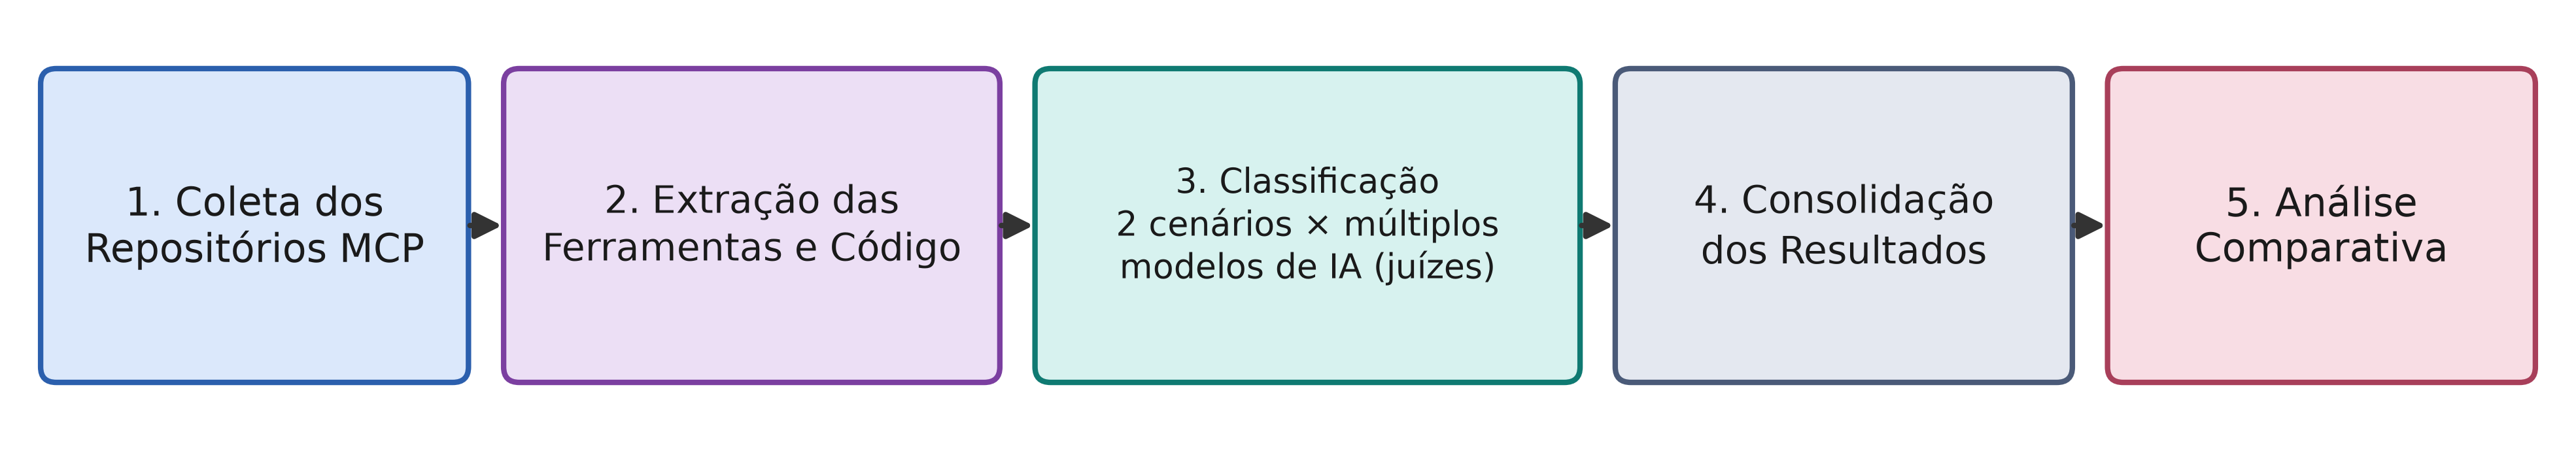
\includegraphics[width=1\linewidth]{./images/metodologia_v7.png}
    \caption{Fluxo metodológico adotado na pesquisa}
    \label{fig:metodologia}
\end{figure}

\subsection{Coleta dos Repositórios MCP}
\label{subsec:coleta}

A primeira etapa consiste na construção do conjunto de dados que \textcolor{orange}{serve} de base para os experimentos. Para isso, foram minerados repositórios públicos relacionados ao ecossistema MCP hospedados no GitHub. O objetivo dessa etapa é identificar implementações reais de servidores MCP que representem o cenário atual.

\textcolor{blue} {As consultas foram construídas a partir dos nomes dos pacotes necessários para a implementação do MCP. Para cada pacote, seu nome foi utilizado como termo de busca nos arquivos de dependências dos projetos. Essa etapa foi realizada por meio da busca de código da API REST do GitHub, que permite localizar repositórios com base em termos presentes no conteúdo de seus arquivos, ainda que a API limite cada consulta a um máximo de 1.000 resultados \cite{BashInTheWild}. Dessa forma, foi necessário dividir a busca em consultas distintas, a fim de ampliar a quantidade de projetos identificáveis. Para isso, foi realizada uma consulta para cada combinação entre o nome da dependência e o respectivo arquivo de dependências em que ela poderia estar declarada. Como essa busca de código não devolve metadados do repositório em si, cada resultado foi complementado por uma consulta separada à API GraphQL do GitHub, de onde vieram o número de estrelas, a condição de \textit{fork} e a linguagem principal usados nos filtros seguintes. Ao final, os repositórios duplicados foram unificados por identificador. Após isto, os que eram \textit{fork} e os que não atingiam o piso mínimo de estrelas, ou cuja linguagem principal não estava entre as linguagens-alvo do estudo, foram removidos.}

Para garantir a relevância e a maturidade dos \textit{softwares} analisados, a coleta foi restrita a repositórios que possuam no mínimo 100 estrelas (\textit{stars}). A adoção desse limiar fundamenta-se em estudos de mineração de repositórios que identificam o número de estrelas como uma medida direta de popularidade, sendo 100 estrelas um marco estatístico comum para filtrar projetos experimentais ou de baixo valor agregado, conhecidos como \textit{toy repositories} \cite{Borges2016}. Ao final, foram selecionados os 206 servidores mais populares encontrados e que possuíam ao menos uma tool, dobrando a amostra utilizada no estudo de Hasan et al. (2026)\nocite{2026arXiv260214878M} para ampliar a cobertura do ecossistema investigado.

\textcolor{orange}{A Figura \ref{fig:fluxo-etapa1} detalha o funcionamento interno dessa etapa. A mineração é realizada via API REST de busca de código do GitHub, segmentada por termos: cada combinação entre um sinal de dependência (por exemplo, \texttt{@modelcontextprotocol/sdk}) e um arquivo de manifesto onde esse sinal poderia estar declarado (por exemplo, \texttt{package.json}) gera uma sub-consulta independente; a linguagem não faz parte dessa segmentação e só é determinada depois, na hidratação de cada candidato. Cada repositório encontrado é então hidratado via GraphQL para a obtenção de seus metadados de linguagem principal e número de estrelas, informações não disponíveis diretamente na busca de código. Em seguida, os repositórios são unificados por identificador (removendo duplicatas encontradas por mais de uma sub-consulta) e submetidos à verificação de elegibilidade descrita acima. Os repositórios aprovados são ordenados por número de estrelas, e os mais relevantes são extraídos para compor a amostra final.}

\begin{figure}[H]
    \centering
    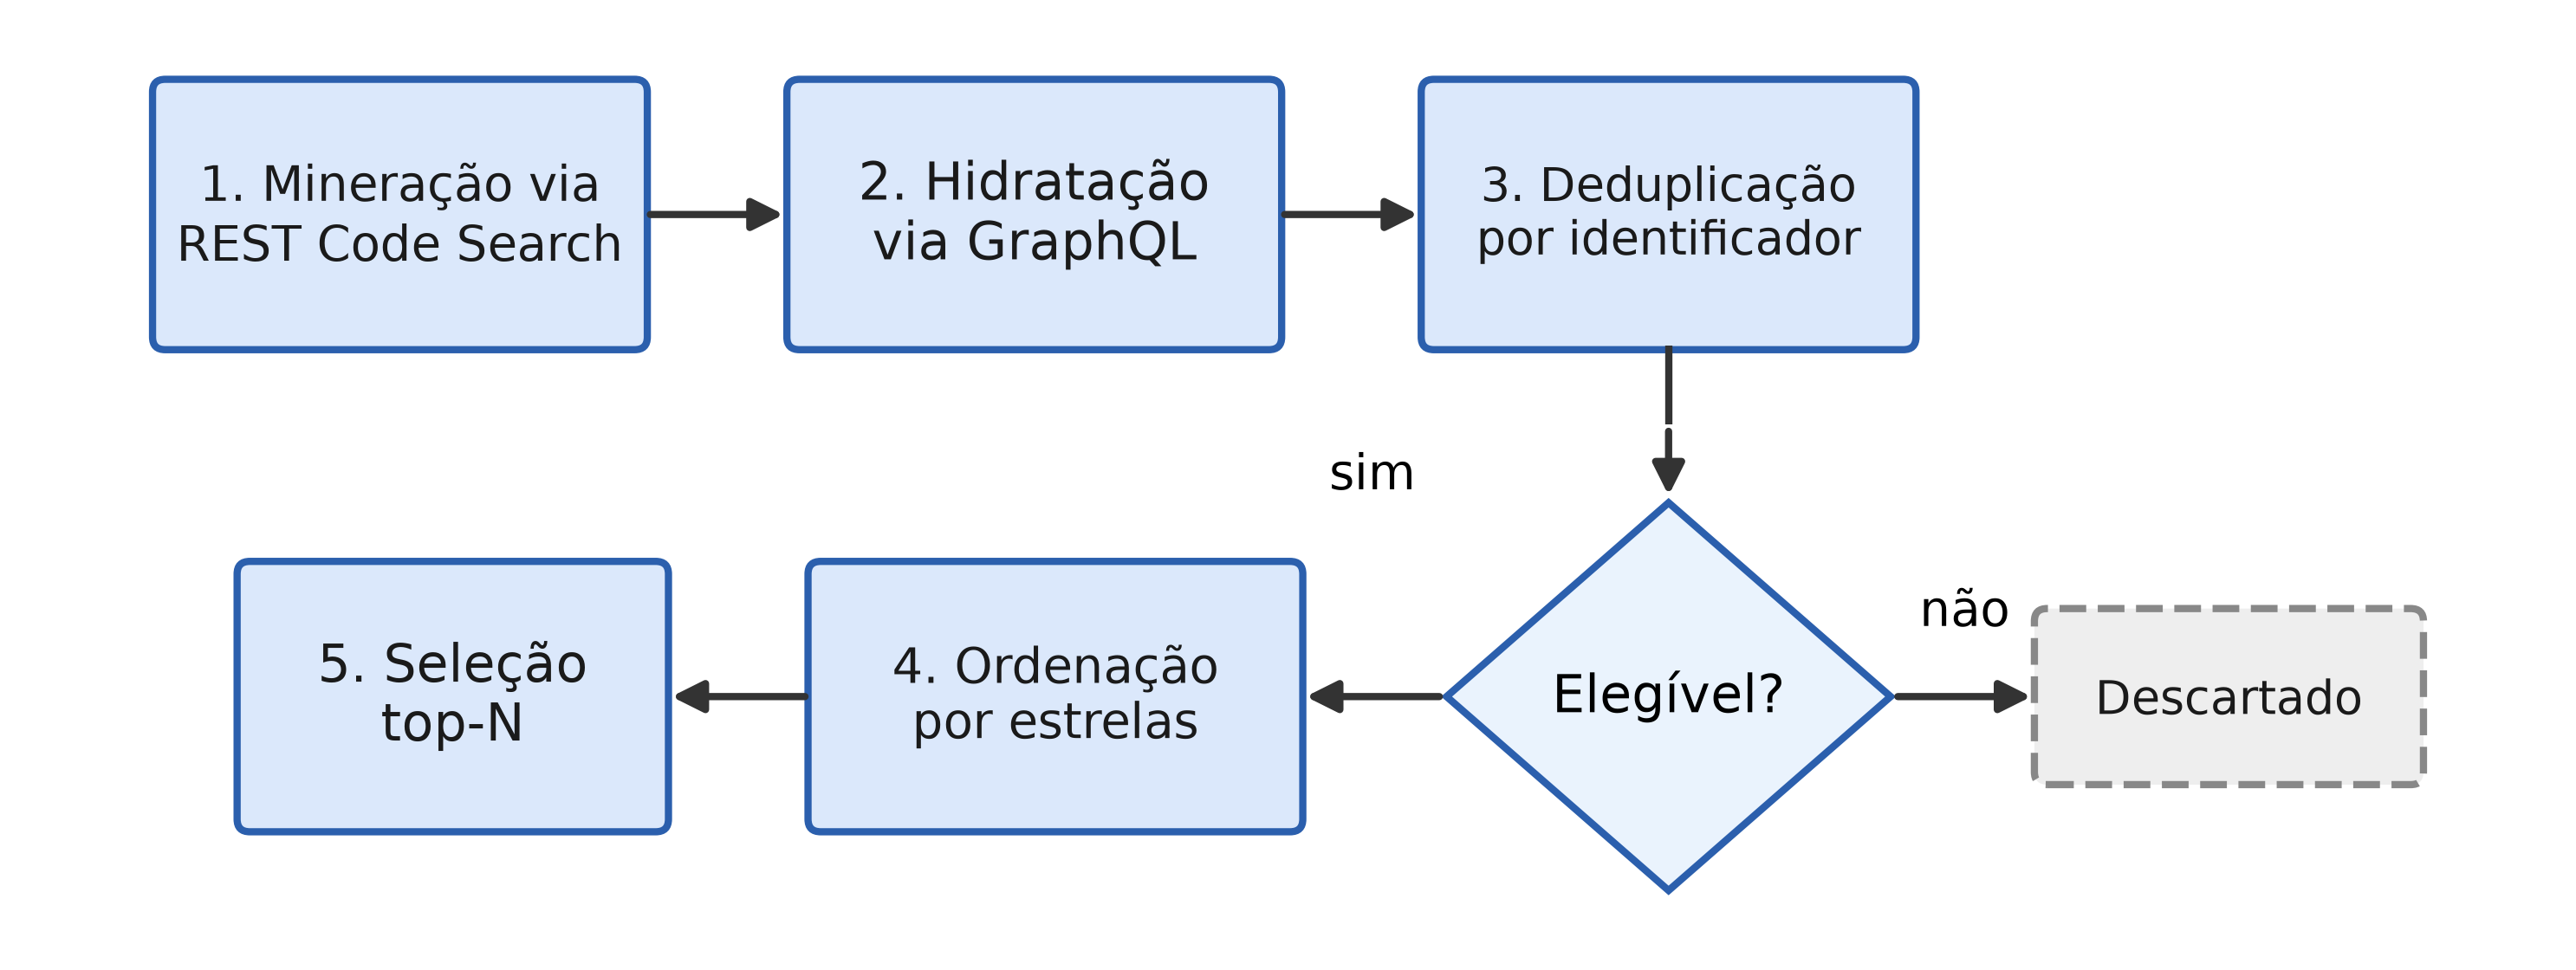
\includegraphics[width=1\linewidth]{./images/fluxo_etapa1_detalhado.png}
    \caption{Funcionamento detalhado da Etapa 1 (Coleta dos Repositórios)}
    \label{fig:fluxo-etapa1}
\end{figure}

\textcolor{orange}{A busca por sinais de manifesto devolveu 12.058 candidatos brutos, todos provenientes de arquivos de dependência (\texttt{package.json}, \texttt{pyproject.toml}, \texttt{pom.xml} e equivalentes), únicos após a deduplicação por identificador. A Tabela \ref{tab:funil-coleta} apresenta o funil de atrito aplicado sobre esse conjunto: o filtro de elegibilidade (repositório não ser \textit{fork}, possuir pelo menos 100 estrelas e estar em uma das linguagens-alvo) reduziu esse conjunto para 723 repositórios.}

\begin{table}[H]
\centering
\caption{Funil de atrito da Etapa 1 (Coleta dos Repositórios MCP)}
\label{tab:funil-coleta}
\begin{tabular}{|p{0.6\linewidth}|r|r|}
\hline
\textbf{Etapa do filtro} & \textbf{Repositórios} & \textbf{\% do bruto} \\ \hline
Candidatos brutos (busca por manifesto) & 12.058 & 100,0\% \\ \hline
Aprovados no filtro (não-fork, estrelas $\geq$ mínimo, linguagem-alvo) & 723 & 6,0\% \\ \hline
Selecionados (qualificados pelo laço de \textit{backfill}) & 206 & 1,7\% \\ \hline
\end{tabular}
\end{table}

\textcolor{orange}{Diferentemente de um corte simples pelas 206 posições mais bem colocadas, a seleção final passa por um laço de preenchimento (\textit{backfill}): um repositório só permanece selecionado se, após a Etapa 2, confirmar pelo menos uma ferramenta; repositórios desqualificados são substituídos pelo próximo candidato do pool ainda não tentado, e o processo se repete até fechar as 206 vagas ou esgotar o pool. Entre os repositórios selecionados, a distribuição por linguagem principal está longe de ser uniforme, com forte concentração em Python e TypeScript (Tabela~\ref{tab:media-tools-servidor}).}


\subsection{Extração das Ferramentas e do Código Relacionado}
\label{subsec:extracao}

Após a obtenção dos repositórios, cada um foi clonado localmente para permitir a identificação automática das ferramentas
disponibilizadas por cada servidor MCP, chegando ao resultado de 12.171
ferramentas. Para isso, foi desenvolvido um algoritmo de mineração capaz
de percorrer a estrutura dos projetos e localizar as implementações
associadas às ferramentas expostas pelo servidor. Para cada ferramenta
identificada, foram extraídos sua descrição em linguagem natural e sua
localização no código. Um repositório em que nenhuma ferramenta é
localizada é tratado, na prática, como um falso positivo da etapa de
coleta: ele é removido da amostra e substituído pelo próximo candidato
ainda não testado, repetindo-se o processo até completar o número de
repositórios definido para o estudo ou esgotar os candidatos disponíveis\textcolor{orange}{, fechando o mesmo laço de \textit{backfill} descrito na Seção~\ref{subsec:coleta}}.

\textcolor{orange}{A Figura \ref{fig:fluxo-etapa2} detalha o funcionamento interno dessa etapa (clonagem, detecção de ferramentas e construção do grafo de chamadas), incluindo o laço de \textit{backfill} entre Etapas 1 e 2. Cada repositório selecionado é primeiro clonado e então indexado estaticamente: são catalogadas todas as definições de função/método e, por arquivo, os \textit{imports} declarados. Em seguida, aplica-se o padrão estrutural do SDK correspondente à linguagem do repositório para localizar as ferramentas declaradas; se nenhuma ferramenta é encontrada, o repositório é desqualificado e substituído, reentrando no fluxo a partir da clonagem.}

\begin{figure}[H]
    \centering
    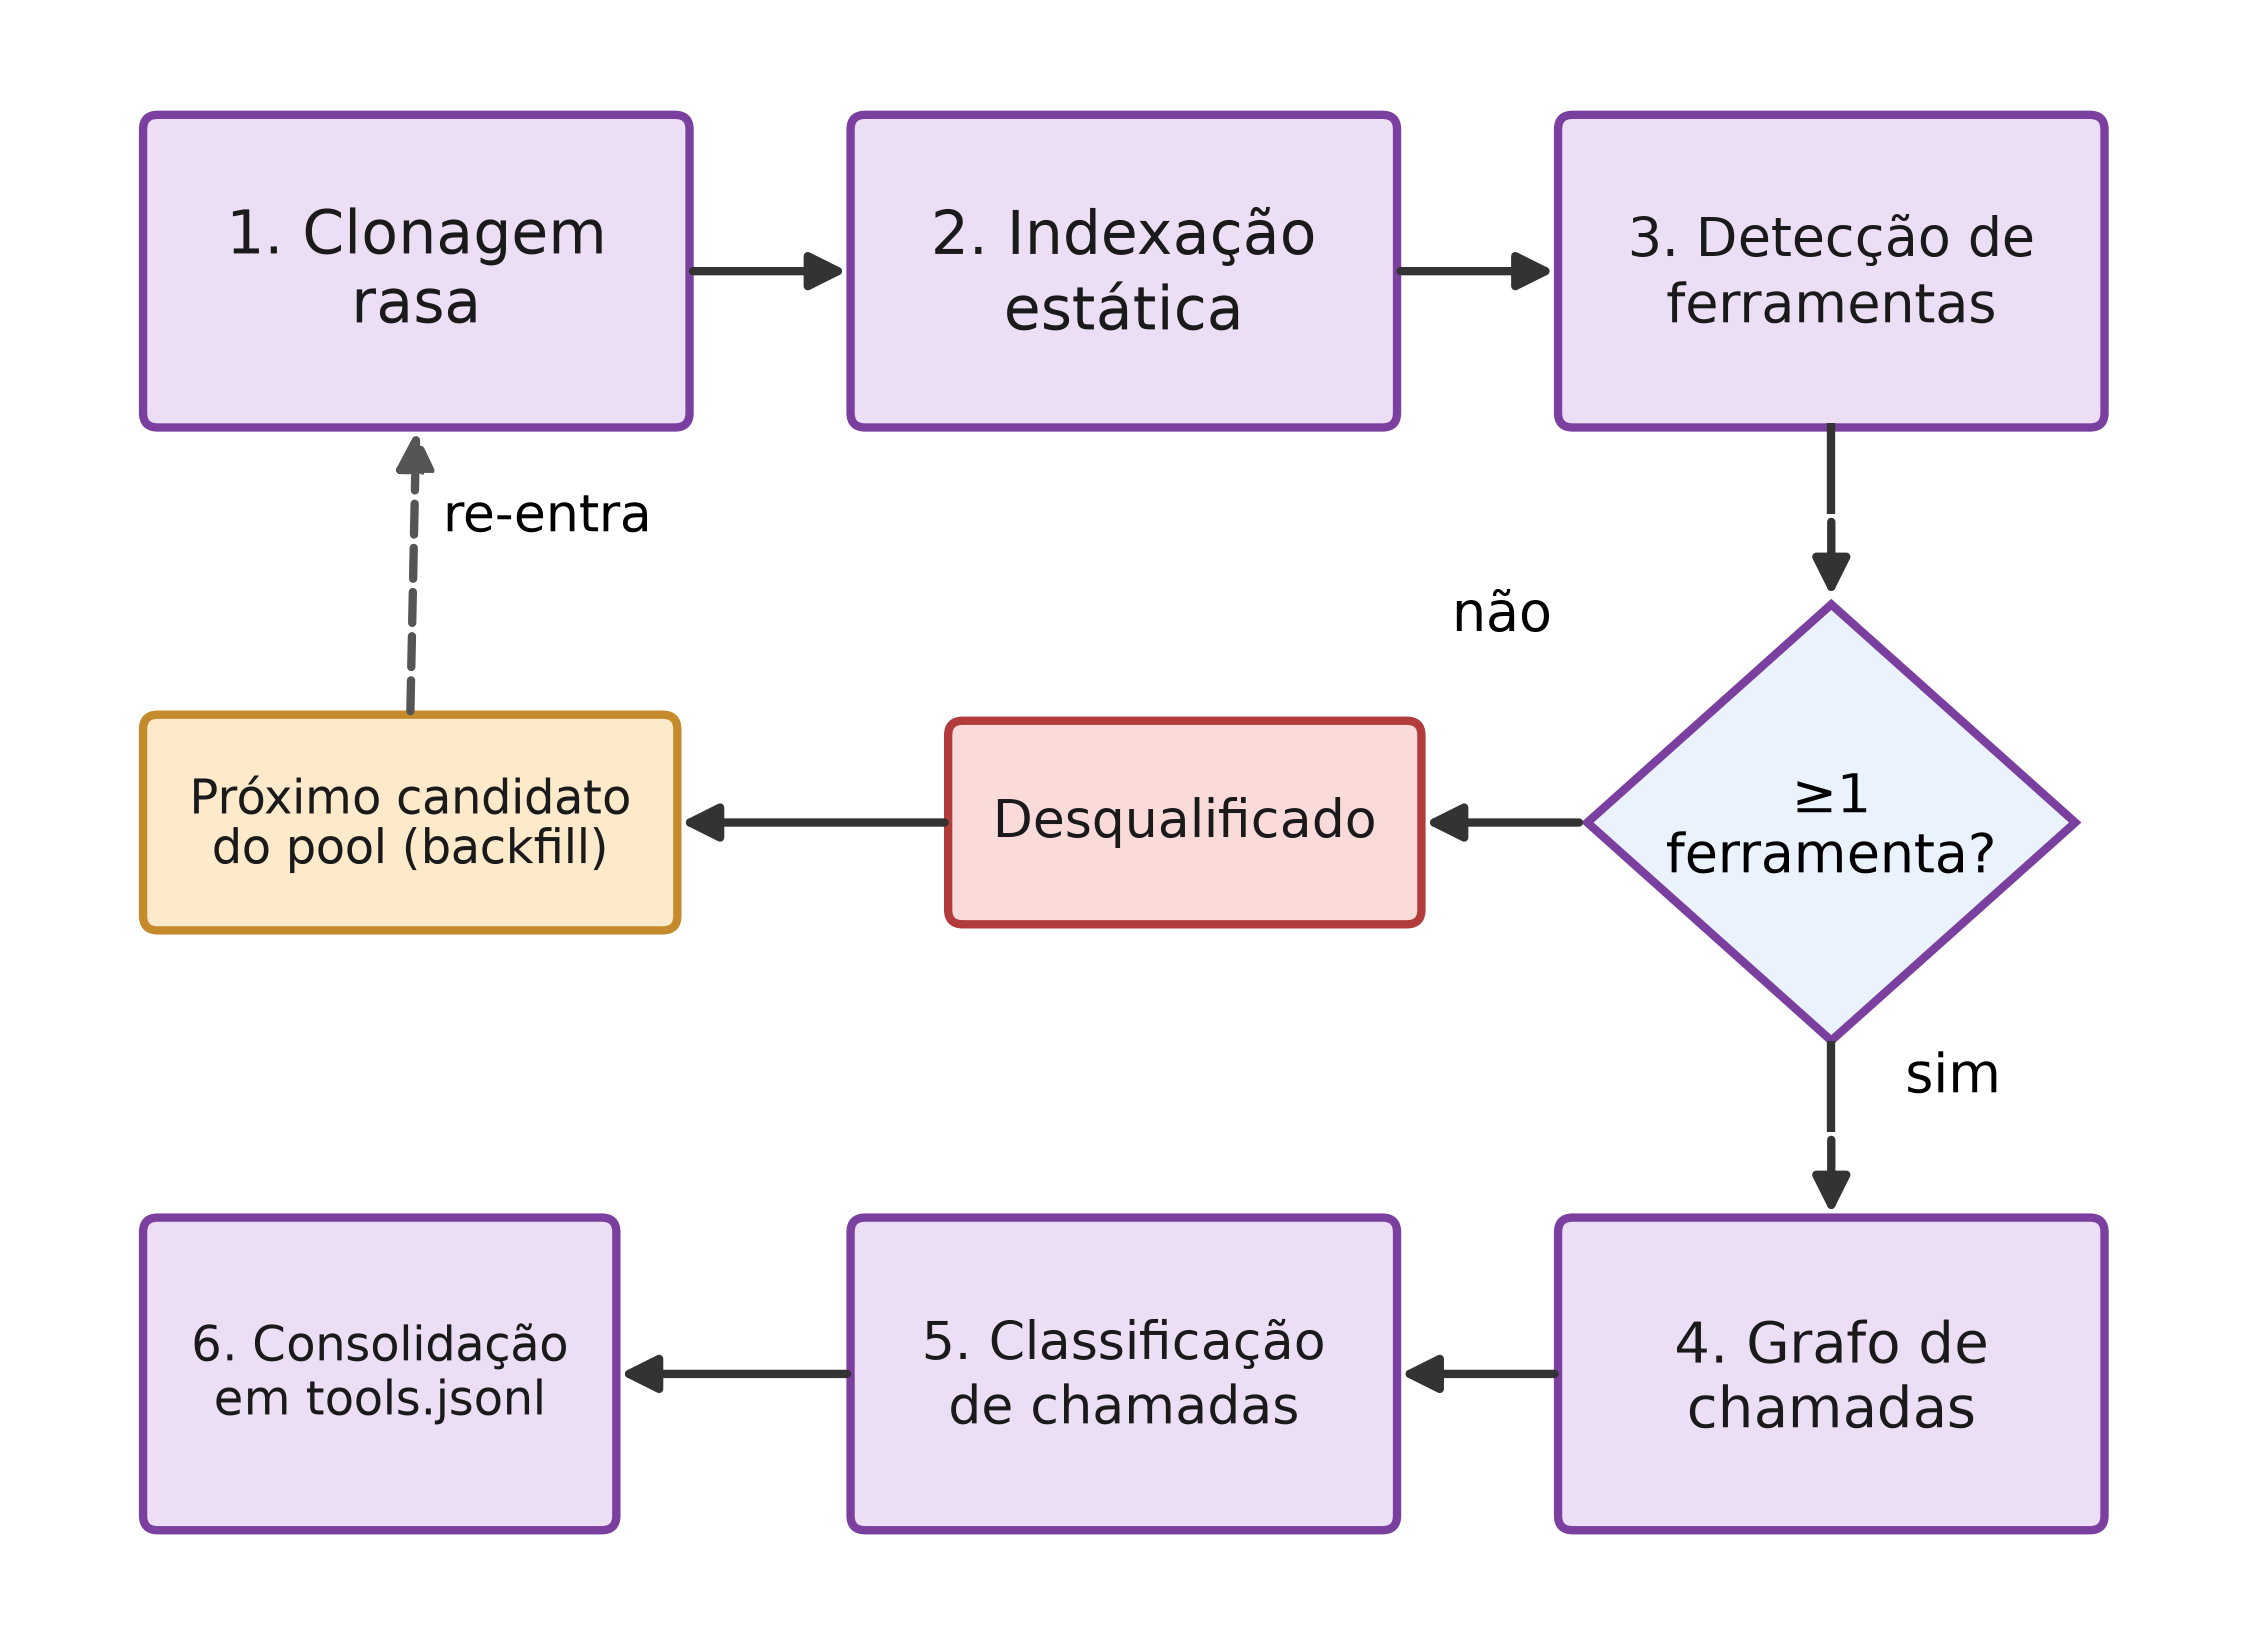
\includegraphics[width=1\linewidth]{./images/fluxo_etapa2_detalhado.png}
    \caption{Funcionamento detalhado da Etapa 2 (Extração das Ferramentas)}
    \label{fig:fluxo-etapa2}
\end{figure}

Em seguida, foi realizada a extração do código relacionado a cada ferramenta. Como os servidores MCP possuem estruturas variadas, extrair apenas o método raiz de uma ferramenta pode não ser suficiente para capturar sua lógica, sendo necessário incluir também os métodos subsequentemente invocados. Para isso, foi construída uma árvore de chamadas (\textit{call graph}) a partir do método inicial\textcolor{orange}{, expandida recursivamente até um limite máximo de três níveis de profundidade}: o próprio método inicial constitui o primeiro nível; os métodos chamados diretamente por ele\textcolor{orange}{, quando resolvidos,} formam o segundo nível; e as chamadas efetuadas a partir destes compõem o terceiro nível. \textcolor{orange}{A limitação da profundidade a três níveis é uma decisão de engenharia, não uma medição prévia de onde termina a lógica relevante de uma ferramenta: ela contém o custo da análise (e do texto eventualmente enviado ao avaliador) e elimina, por construção, qualquer risco de recursão infinita, sem exigir detecção de ciclo separada (ver Apêndice~\ref{apendice:secao} para o detalhamento completo da heurística de resolução).} Um exemplo desse processo é apresentado na Figura \ref{fig:codigoarvore}.

\begin{figure}[H]
    \centering
    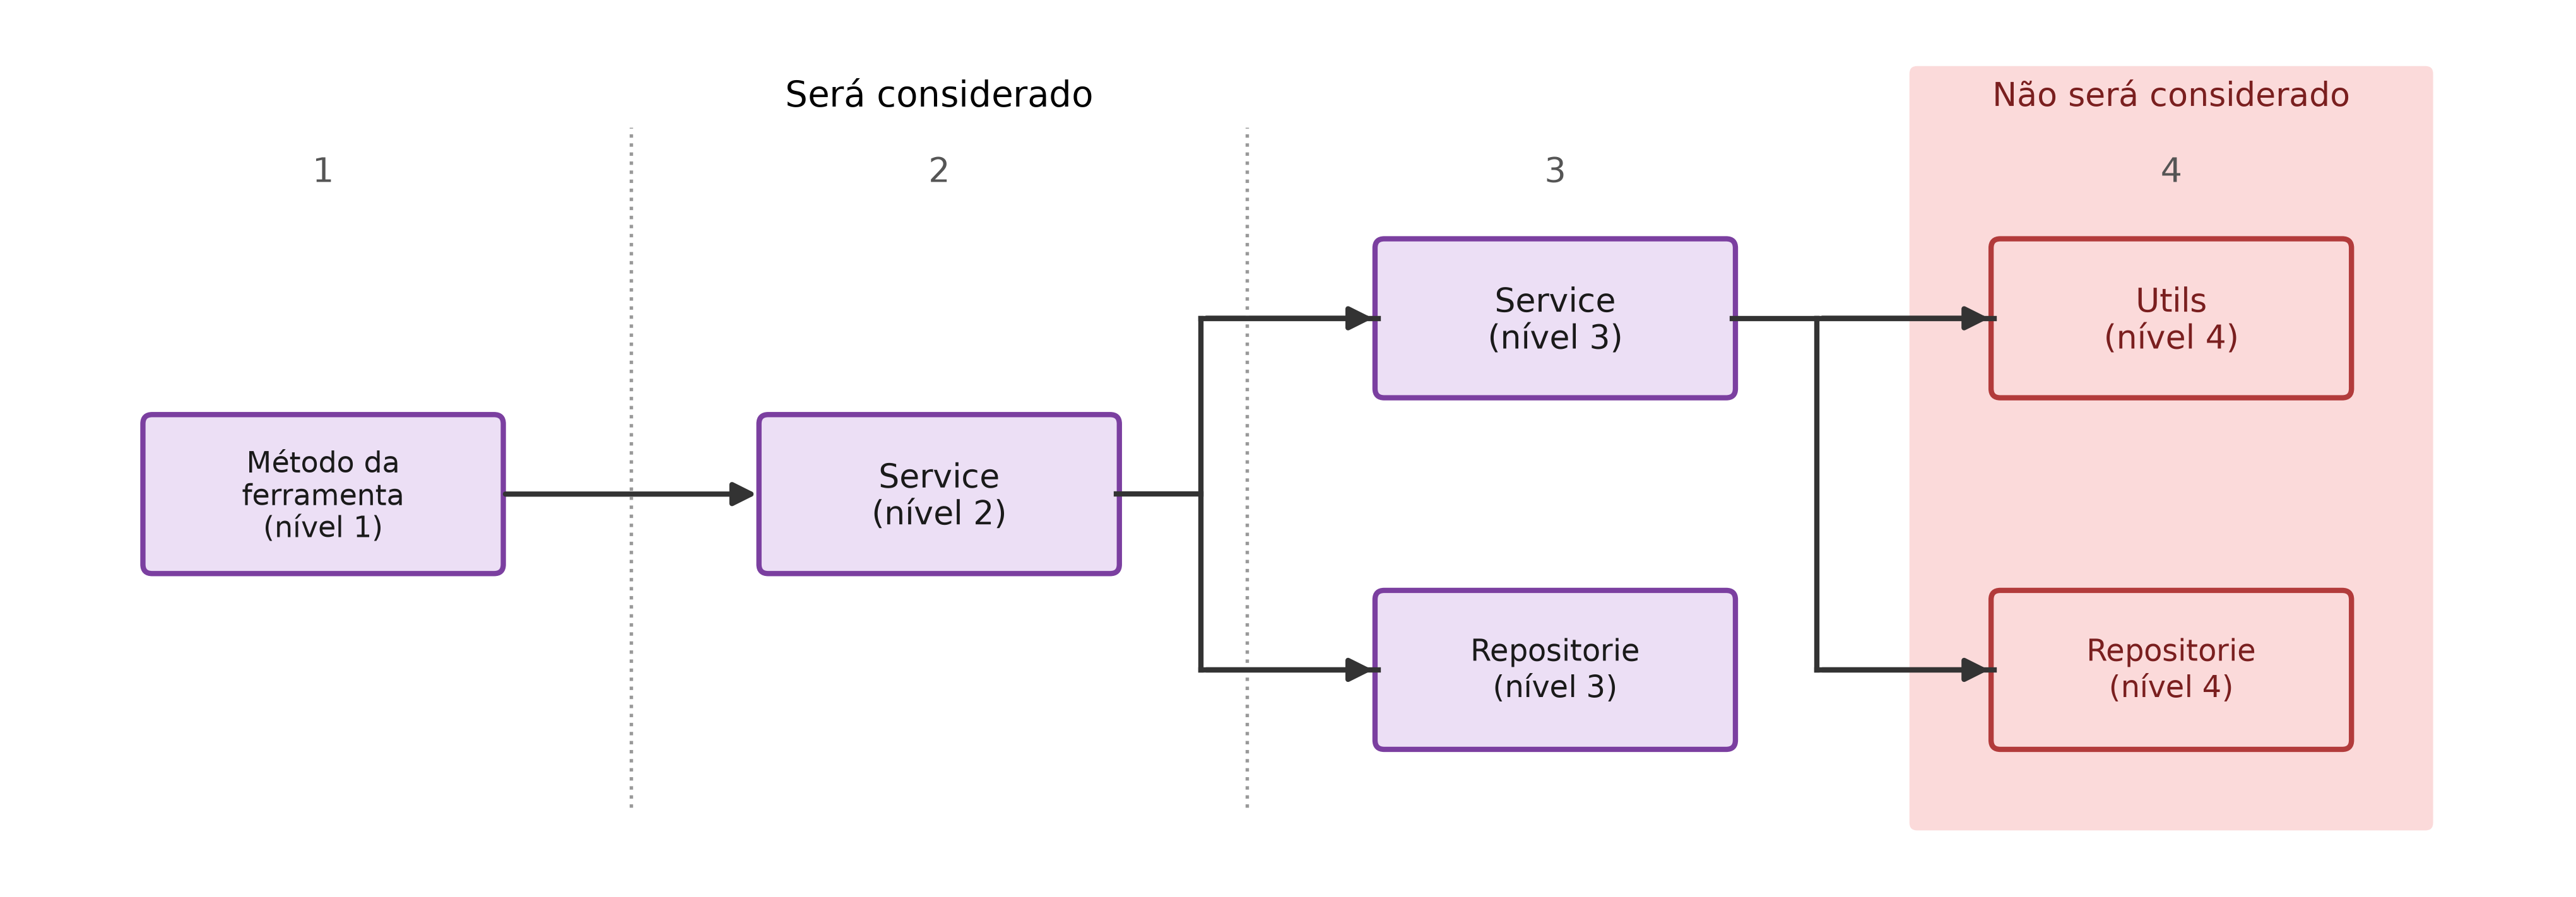
\includegraphics[width=1\linewidth]{./images/arvoreFinal.png}
    \caption{Exemplo de extração da árvore de chamadas de uma ferramenta}
    \label{fig:codigoarvore}
\end{figure}

Ao final desta etapa, foi produzido um conjunto de dados estruturado contendo os servidores MCP analisados e as ferramentas identificadas em cada um deles. Para cada ferramenta, \textcolor{orange}{são armazenadas} sua descrição em linguagem natural e o conjunto de métodos obtido a partir da árvore de chamadas. Esse conjunto de dados \textcolor{orange}{serve} como entrada para as etapas subsequentes da pesquisa, nas quais as ferramentas dos repositórios coletados \textcolor{orange}{são avaliadas} quanto à qualidade de suas descrições, com e sem o uso do código correspondente.

\textcolor{orange}{A Etapa 2 extraiu 12.171 ferramentas dos 206 repositórios selecionados; como a seleção final já incorpora o laço de \textit{backfill}, todo repositório selecionado confirma, por construção, pelo menos uma ferramenta. A distribuição de ferramentas por linguagem segue de perto a distribuição de repositórios vista na coleta, com a mesma concentração em Python e TypeScript e uma assimetria adicional por repositório individual (Tabela~\ref{tab:media-tools-servidor}). Python (79 repositórios, 38,3\%) e TypeScript (45, 21,8\%) concentram 60\% dos repositórios e 85,6\% das ferramentas; nenhum repositório em Kotlin, PHP, Elixir, Lua ou Swift permaneceu na seleção final, pois os candidatos dessas linguagens foram descartados pelo laço de \textit{backfill} por não confirmarem nenhuma ferramenta, ou nunca alcançaram o piso de estrelas dentro do pool.}

\begin{table}[H]
\centering
\caption{Repositórios selecionados e total de ferramentas extraídas, por linguagem}
\label{tab:media-tools-servidor}
\begin{tabular}{|l|r|r|r|}
\hline
\textbf{Linguagem} & \textbf{Repositórios} & \textbf{Tools (total)} & \textbf{Média/repositório} \\ \hline
Python & 79 & 7.251 & 91,78 \\ \hline
TypeScript & 45 & 3.162 & 70,27 \\ \hline
Java & 13 & 793 & 61,00 \\ \hline
C\# & 21 & 423 & 20,14 \\ \hline
Rust & 26 & 276 & 10,62 \\ \hline
Go & 13 & 149 & 11,46 \\ \hline
JavaScript & 6 & 108 & 18,00 \\ \hline
Ruby & 2 & 5 & 2,50 \\ \hline
Dart & 1 & 4 & 4,00 \\ \hline
\textbf{Total} & \textbf{206} & \textbf{12.171} & \textbf{59,08} \\ \hline
\end{tabular}
\end{table}

\textcolor{orange}{A concentração de ferramentas por repositório também é fortemente assimétrica: os três repositórios com mais ferramentas respondem, sozinhos, por 46,6\% de todo o conjunto de dados (20,4\%, 18,4\% e 7,8\%, respectivamente), um deles em TypeScript, os outros dois em Python. Esse resultado eleva consideravelmente a média de ferramentas por repositório nessas duas linguagens e deve ser considerado ao interpretar médias agregadas por linguagem.}




\subsection{Classificação das tools por diferentes modelos de IA}

Na terceira etapa, utilizando as \textit{tools} coletadas nas etapas anteriores, \textcolor{orange}{é conduzido} um experimento comparativo estruturado em dois cenários de avaliação\textcolor{orange}{, executados} em diferentes modelos de IA. No primeiro cenário, as descrições das ferramentas \textcolor{orange}{são avaliadas} com base em seu conteúdo em linguagem natural. No segundo, essas mesmas descrições \textcolor{orange}{são avaliadas} em conjunto com informações extraídas do código correspondente. Essa estratégia permite identificar o impacto da inclusão do contexto de implementação na avaliação da qualidade das descrições.

\textcolor{orange}{A Figura \ref{fig:fluxo-etapa3} detalha o funcionamento interno dessa etapa. Para cada ferramenta, são montados os dois cenários de avaliação descritos acima; cada cenário gera um \textit{payload} contendo o nome da ferramenta, seu servidor de origem, a descrição e, quando aplicável, o código de contexto, enviado a cada juiz habilitado de forma concorrente. As respostas dos juízes podem resultar em uma avaliação concluída, em uma recusa de segurança do provedor, ou em um erro técnico durante o processamento. As duas primeiras são gravadas no arquivo de resultados e recebem uma entrada de \textit{checkpoint}, permitindo retomar a execução sem repetir avaliações já concluídas; o erro técnico não gera registro de resultado nem entrada de \textit{checkpoint}, apenas um registro em um log de erros separado, e é reprocessado automaticamente na rodada seguinte.}

\begin{figure}[H]
    \centering
    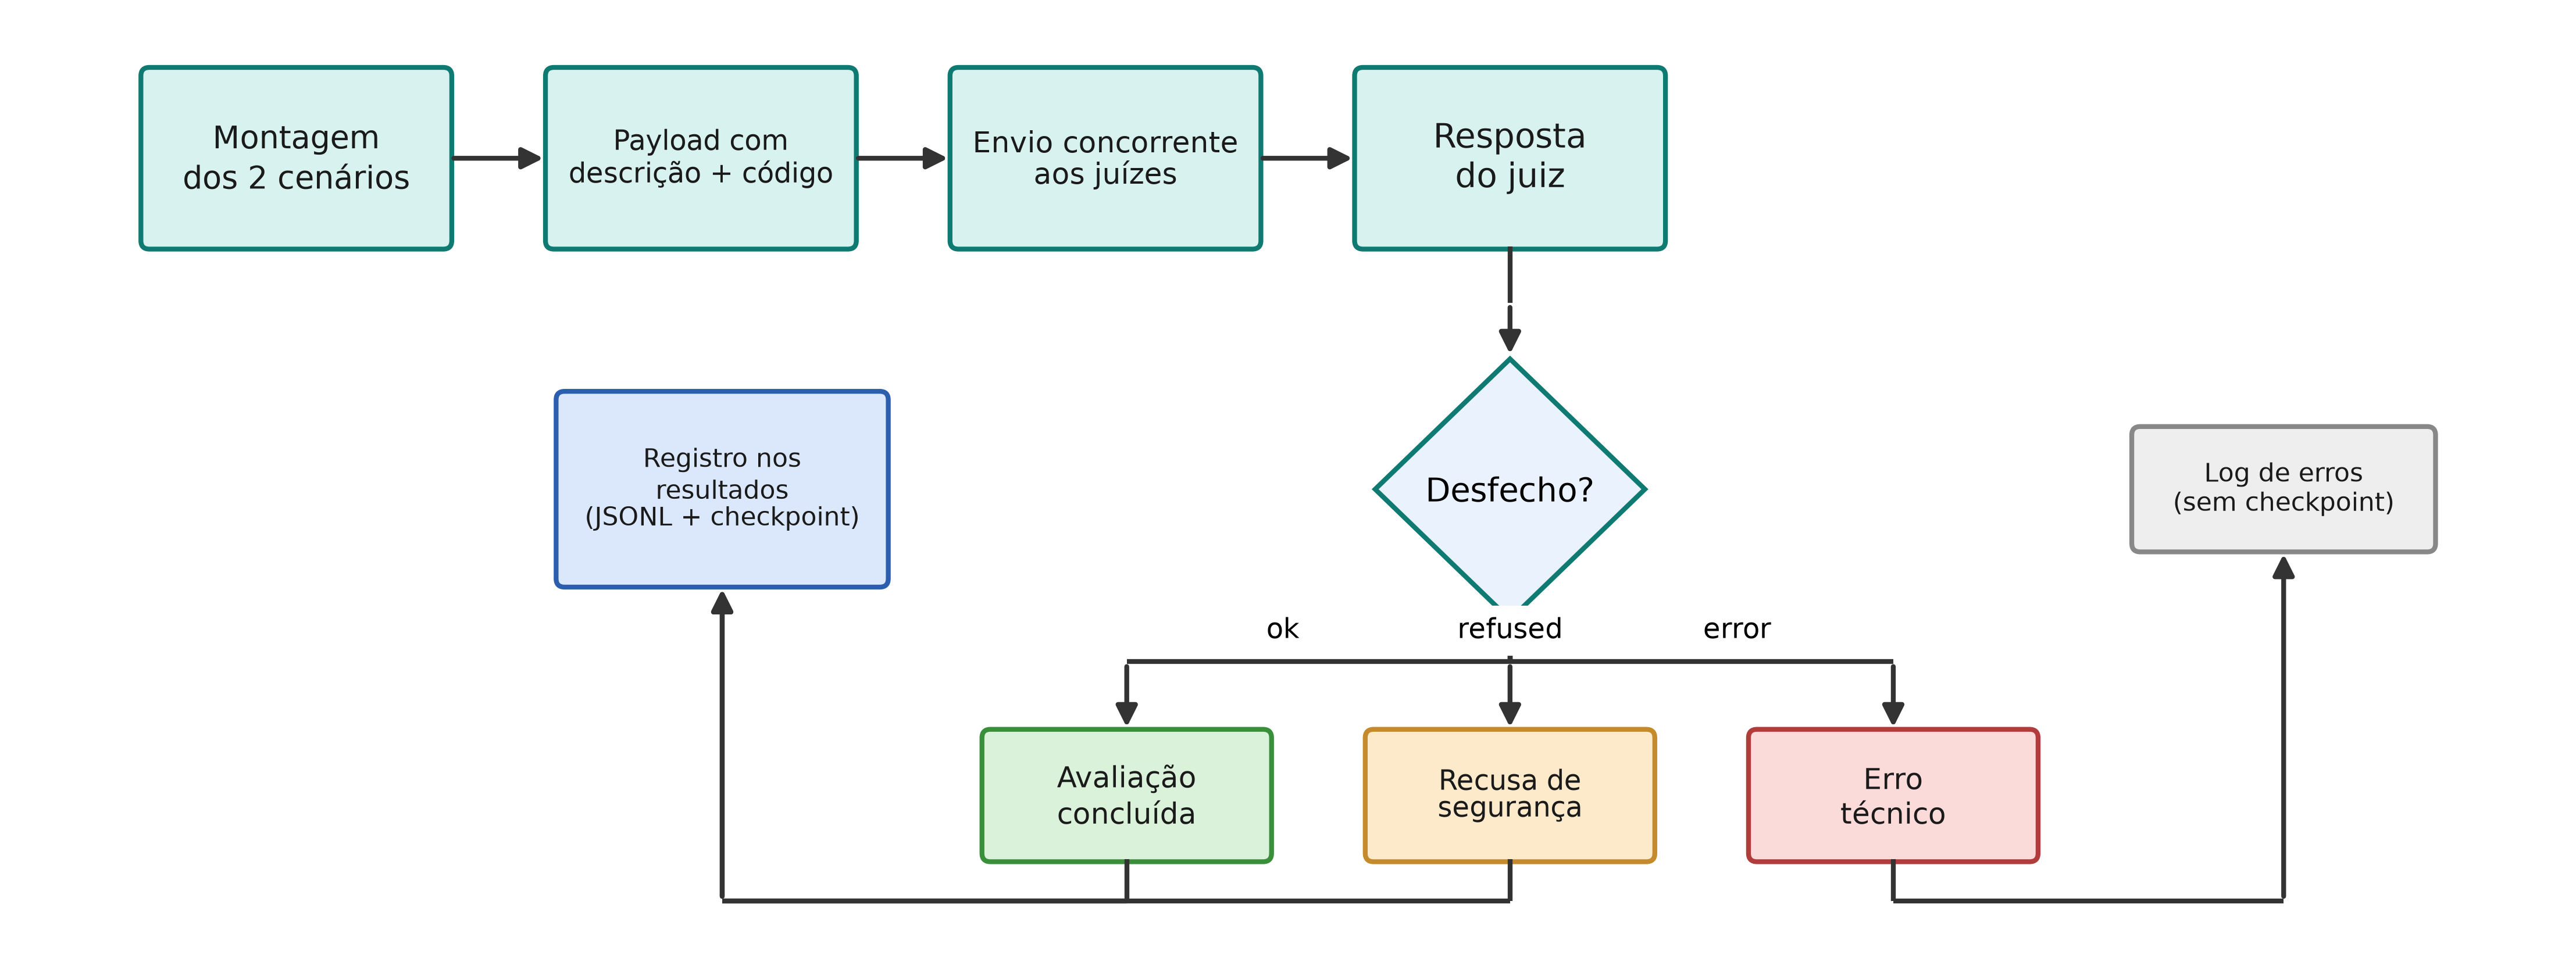
\includegraphics[width=1\linewidth]{./images/fluxo_etapa3_detalhado.png}
    \caption{Funcionamento detalhado da Etapa 3 (Classificação das Ferramentas)}
    \label{fig:fluxo-etapa3}
\end{figure}

\textcolor{orange}{Três modelos de linguagem atuam como juízes neste experimento: DeepSeek-V4.1-Flash e Gemini 3.5 Flash-Lite, acessados via API de seus respectivos provedores, e Qwen3-14B, executado localmente via Ollama. A escolha combina deliberadamente modelos de proveniências distintas (duas famílias de provedores \textit{cloud} distintas, mais um modelo local) e regimes de custo distintos (um modelo pago, um gratuito por \textit{free tier}, um sem custo de API por rodar localmente), reduzindo o risco de que um padrão observado seja específico de um único provedor ou arquitetura, e mantendo o custo do experimento administrável diante do volume de milhares de ferramentas avaliadas em dois cenários. A comparação entre os três juízes é tratada na Seção~\ref{sec:resultados} como um achado em si, não como um pressuposto do desenho experimental: modelos distintos podem reagir de forma diferente à inclusão do código, e o experimento é construído para tornar essa diferença observável, não para assumi-la.}

Em ambos os cenários, a avaliação \textcolor{orange}{é conduzida} com base na rubrica proposta por Hasan et al. (2026)\nocite{2026arXiv260214878M}, composta por seis componentes: \textit{Purpose}, que avalia a clareza com que a descrição comunica a finalidade da ferramenta; \textit{Guidelines}, que verifica se existem orientações sobre quando e como utilizá-la; \textit{Limitations}, que analisa a explicitação de restrições, premissas ou casos de falha; \textit{Parameter Explanation}, que mede a qualidade da documentação dos parâmetros de entrada; \textit{Length and Completeness}, que avalia o nível de detalhamento e cobertura da descrição; e \textit{Examples}, que verifica a presença de exemplos de utilização. Cada componente recebe uma pontuação em uma escala Likert de cinco pontos, sendo posteriormente utilizada para identificar deficiências associadas aos respectivos \textit{smells} descritos pelos autores.

\textcolor{orange}{Em ambos os cenários, os modelos de linguagem atuam como o mesmo avaliador (\textit{LLM-as-a-Judge}), recebendo as descrições das ferramentas e atribuindo as seis pontuações da rubrica acima.} No primeiro cenário\textcolor{orange}{, essa avaliação} é realizada sem qualquer acesso à implementação da funcionalidade analisada. No segundo cenário, \textcolor{orange}{o mesmo avaliador recebe adicionalmente} o código correspondente, \textcolor{orange}{ isto é, os trechos de código-fonte reunidos pela árvore de chamadas construída na Seção~\ref{subsec:extracao}}. Dessa forma, o avaliador \textcolor{orange}{pode} confrontar a descrição fornecida com aspectos observáveis da implementação, verificando a existência de omissões, inconsistências ou informações potencialmente enganosas que não seriam perceptíveis apenas pela análise da descrição.


\subsection{\textcolor{orange}{Consolidação dos Resultados por Cenário}}
\label{subsec:consolidacao}

Concluída a etapa de classificação, os resultados produzidos nos dois cenários experimentais \textcolor{orange}{são coletados e estruturados} em uma base de dados unificada. Para cada ferramenta analisada, \textcolor{orange}{são armazenados} identificadores que \textcolor{orange}{permitem} sua associação ao servidor MCP de origem, bem como os resultados obtidos nos cenários com e sem a inclusão de informações provenientes do código, além de qual modelo de IA foi utilizado na avaliação.

A base de dados resultante \textcolor{orange}{contém} os escores atribuídos pelo modelo para cada dimensão de qualidade avaliada, além das classificações finais produzidas em cada execução do experimento. Dessa forma, cada ferramenta \textcolor{orange}{possui} dois conjuntos de resultados por modelo\textcolor{orange}{, diretamente vinculados} à mesma descrição, diferindo apenas pela presença ou ausência das informações extraídas do código. Essa organização \textcolor{orange}{estabelece} um relacionamento direto entre as avaliações realizadas sobre uma mesma ferramenta, preservando o pareamento necessário para as análises estatísticas subsequentes e possibilitando a comparação consistente dos resultados obtidos nos dois cenários experimentais.

\textcolor{orange}{A partir dessa base consolidada, é identificado um subconjunto adicional de ferramentas, denominado amostra de divergência confirmada, utilizado como base para a análise qualitativa descrita na Seção~\ref{subsec:analise-comparativa}. Uma ferramenta integra essa amostra quando, para pelo menos uma dimensão da rubrica, TODOS os juízes que a avaliaram atribuem notas diferentes entre o cenário sem código e o cenário com código, caracterizando um consenso de divergência entre os avaliadores. Para cada ferramenta selecionada, a amostra de divergência confirmada reúne a justificativa (\textit{reasoning}) de cada juiz nos dois cenários e o trecho de código correspondente, reconstruído pelo mesmo mecanismo descrito na Seção~\ref{subsec:extracao}.}


\subsection{Análise Comparativa dos Experimentos}
\label{subsec:analise-comparativa}

Na etapa final, os resultados obtidos \textcolor{orange}{são analisados} com o objetivo de identificar diferenças entre os dois cenários de avaliação. Essa análise busca validar se a utilização do código de fato altera os resultados da avaliação das descrições, além de identificar quais atributos da rubrica utilizada para avaliar a qualidade são mais e menos impactados pela adição do código.

Inicialmente, \textcolor{orange}{realiza-se} uma análise por meio do cálculo de medidas como média, mediana e desvio-padrão dos escores atribuídos a cada dimensão de qualidade avaliada, para identificar se \textcolor{orange}{há} diferença numérica nos resultados gerados com e sem o contexto do código das ferramentas MCP, atendendo ao objetivo específico (ii) desta pesquisa. A partir dessa comparação, é possível avaliar quais atributos \textcolor{orange}{são} mais afetados pela inserção do contexto técnico. \textcolor{orange}{Aplica-se} também o Teste de Postos Sinalizados de Wilcoxon \cite{wilcoxon1945individual}, \textcolor{orange}{individualmente} para cada dimensão de qualidade, a fim de verificar se as diferenças observadas entre as avaliações são estatisticamente significativas, concluindo o objetivo específico (iii). O teste \textcolor{orange}{é aplicado} separadamente para cada modelo de linguagem utilizado, permitindo verificar se o efeito da inclusão do código se mantém consistente entre diferentes avaliadores. Como as duas avaliações são realizadas sobre a mesma ferramenta, o teste é adequado por considerar amostras pareadas e não exigir a suposição de normalidade dos dados. Os resultados dessa análise \textcolor{orange}{fornecem} as evidências empíricas necessárias para apoiar ou refutar a hipótese de que a incorporação do contexto técnico amplia a capacidade de detecção de \textit{smells} em descrições de ferramentas MCP.

\textcolor{orange}{Formalmente, para cada dimensão da rubrica e cada juiz, testa-se a hipótese nula de que a distribuição das diferenças pareadas entre os escores do cenário com código e do cenário sem código é simétrica em torno de zero, contra a hipótese alternativa de que a inclusão do código desloca essa distribuição. Como o teste é repetido para as seis dimensões da rubrica em cada juiz, \textcolor{orange}{avalia-se} a necessidade de correção para comparações múltiplas antes de reportar significância. Pares de ferramentas em que os dois cenários recebem exatamente o mesmo escore (diferença zero) são descartados do cálculo do teste, conforme o tratamento padrão de empates do Teste de Wilcoxon; a proporção de pares descartados por esse motivo \textcolor{orange}{é reportada} junto com o resultado do teste, por dimensão, como indicador adicional do quanto a inclusão do código muda ou não a nota atribuída. Essa análise é implementada no mesmo script de análise dedicado da subseção anterior, a partir da base consolidada ali descrita.}

\textcolor{orange}{Como leitura complementar, mais descritiva, da magnitude dessas diferenças, aplica-se também uma análise de transição de quartil: a distribuição de escores no cenário sem código é dividida em quartis, por dimensão da rubrica, a partir da média das notas atribuídas pelos modelos de IA utilizados; cada ferramenta é então reclassificada conforme a faixa de quartil em que seu escore médio no cenário com código se enquadraria nessa mesma distribuição de referência. Essa reclassificação permite reportar a proporção de ferramentas que mantêm, sobem ou descem de faixa de quartil entre os dois cenários, uma leitura que captura mudanças de posição relativa mesmo quando a diferença de escore absoluta é pequena.}

\textcolor{orange}{Complementando a análise estatística acima, conduz-se uma análise qualitativa sobre a amostra de divergência confirmada (Seção~\ref{subsec:consolidacao}), com o objetivo de caracterizar não apenas quais dimensões da rubrica são mais afetadas pela inclusão do código, mas também que tipo de informação o código tende a revelar, e que a descrição, isoladamente, não comunica. Essa análise segue as fases de uma análise temática \cite{braunclarke2006thematic}, complementadas por uma etapa final de análise de conteúdo dirigida \cite{hsiehshannon2005content}, conforme ilustrado na Figura~\ref{fig:fluxo-qualitativa}.}

\begin{figure}[H]
    \centering
    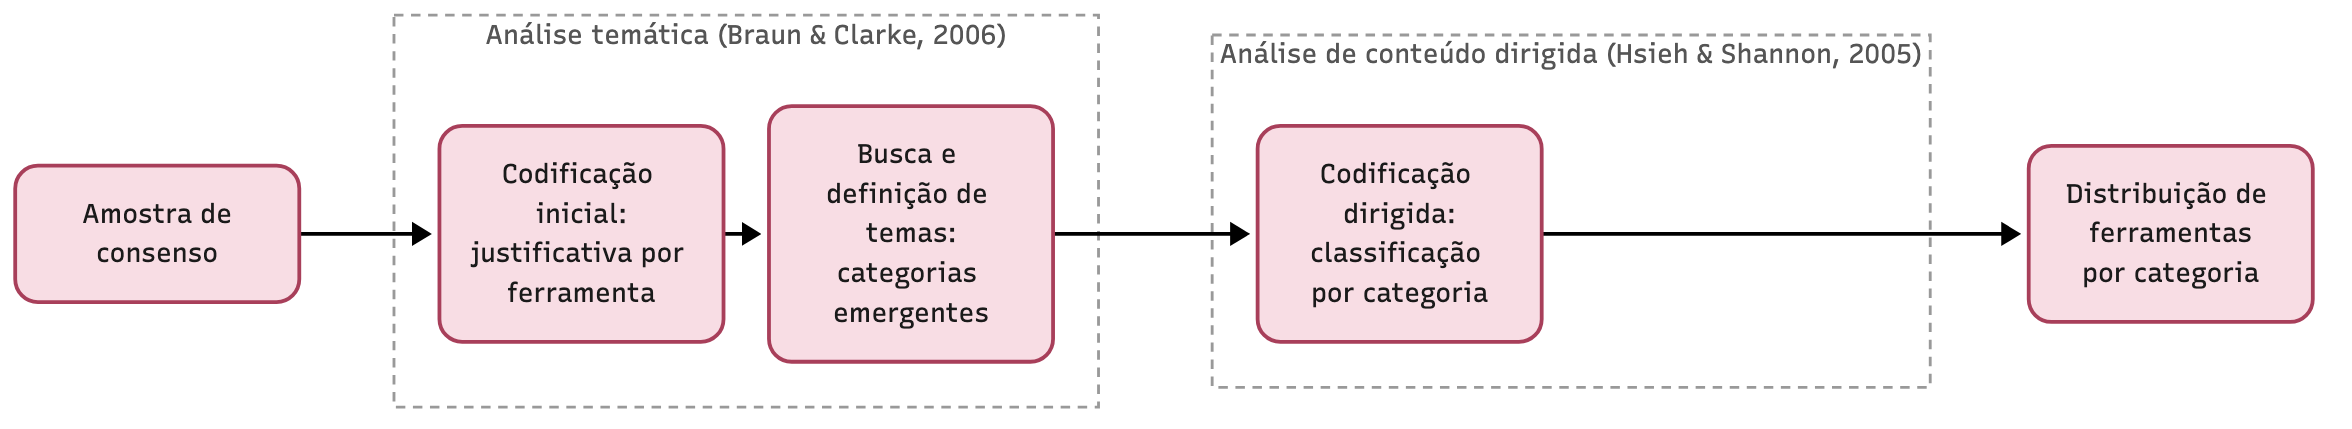
\includegraphics[width=1\linewidth]{./images/fluxo_analise_qualitativa_detalhado.png}
    \caption{Fluxo detalhado da análise qualitativa sobre a amostra de divergência confirmada}
    \label{fig:fluxo-qualitativa}
\end{figure}

\textcolor{orange}{Nas duas fases iniciais da análise temática, familiarização com os dados e codificação inicial \cite{braunclarke2006thematic}, para cada ferramenta da amostra de divergência confirmada um modelo de linguagem (Gemini) é instruído a ler a justificativa (\textit{reasoning}) de cada juiz nos dois cenários para o(s) componente(s) em que houve divergência, confrontá-la com o trecho de código correspondente, e sintetizar, em inglês, uma única justificativa concisa explicando o que o código revelou e que a descrição não comunicava: uma omissão de parâmetro, um comportamento ou formato de saída não documentado, uma limitação não divulgada, ou uma contradição direta entre descrição e implementação. O modelo é explicitamente instruído a não inferir uma conexão entre a mudança de nota e um achado do código quando a justificativa original do juiz não oferecer evidência concreta para isso, registrando essa ausência de evidência em vez de inventar uma explicação plausível; o texto completo do \textit{prompt} utilizado encontra-se no Apêndice~\ref{apendice:secao-prompts}.}

\textcolor{orange}{Nas três fases seguintes, busca, revisão e definição dos temas \cite{braunclarke2006thematic}, é realizada uma única chamada a um modelo de linguagem (DeepSeek), contendo o conjunto completo de justificativas produzidas na fase anterior, com o objetivo de identificar, de baixo para cima e sem partir de uma lista pré-definida, as categorias recorrentes que descrevem o mecanismo pelo qual o código revela uma inconsistência, por exemplo um parâmetro documentado como configurável mas na realidade fixado no código, ou uma estrutura de retorno mais rica do que a descrição sugere. O uso de um modelo distinto do Gemini nesta fase é uma decisão técnica, não metodológica: o volume de texto enviado numa única chamada excede o teto de taxa do tier gratuito do Gemini, enquanto o DeepSeek, já integrado ao projeto como um dos juízes, não impõe esse limite. Cada categoria resultante é delimitada por uma descrição textual própria e exige estar fundamentada em ocorrências de mais de uma ferramenta, de modo a não introduzir uma categoria em função de um único caso idiossincrático (\textit{prompt} completo no Apêndice~\ref{apendice:secao-prompts}).}

\textcolor{orange}{Concluída a análise temática, aplica-se uma análise de conteúdo dirigida \cite{hsiehshannon2005content}: o conjunto fixo de categorias produzido na fase anterior é utilizado para classificar cada ferramenta da amostra de divergência confirmada, permitindo que uma mesma justificativa seja associada a mais de uma categoria, ou a nenhuma quando não houver correspondência, já que um mesmo achado de código pode evidenciar mais de um tipo de omissão simultaneamente. Diferentemente da fase de definição dos temas, na qual o conjunto completo de justificativas é analisado de uma só vez para permitir que os padrões emerjam por comparação entre casos, essa classificação é realizada individualmente, uma ferramenta por vez: ao se solicitar a um modelo de linguagem que classifique milhares de itens em uma única resposta, o desempenho do modelo tende a degradar-se para os itens posicionados no meio da lista \cite{liu2024lost}, risco que a classificação item a item elimina por construção (\textit{prompt} completo no Apêndice~\ref{apendice:secao-prompts}).}

\textcolor{orange}{A classificação dirigida produzida na etapa anterior é, por sua vez, submetida a uma verificação manual sobre uma amostra de ferramentas, cujo tamanho é determinado pela Fórmula de Cochran para populações de tamanho conhecido \cite{chaokromthong2021sample} (Equação~\ref{eq:cochran}), que fornece o número mínimo de casos a observar sem prejudicar a validade do estudo. De forma semelhante ao estudo de Hasan et al. (2026) \nocite{2026arXiv260214878M}, utiliza-se uma taxa de 95\% de nível de confiança (Z = 1,96), uma proporção de população estimada de 0,5 (p) e 10\% de margem de erro ($\varepsilon$), o que leva ao resultado de n = 96, arredondado para 100 ferramentas.}

\begin{equation}
n = \frac{\dfrac{Z^2 p(1 - p)}{\varepsilon^2}}{1 + \left( \dfrac{Z^2 p(1 - p)}{\varepsilon^2 N} \right)}
\label{eq:cochran}
\end{equation}

\textcolor{orange}{A seleção dessas 100 ferramentas é estratificada por categoria de mecanismo, com vagas distribuídas o mais igualmente possível entre as 16 categorias (mais a classificação \texttt{none}) em vez de proporcionalmente à frequência de cada uma, de modo que a amostra não fique concentrada na categoria mais comum da população. Dentro de cada categoria, a seleção prioriza ferramentas de repositórios e de componentes divergentes da rubrica de Hasan et al. (2026) ainda não representados na amostra, para também não concentrar em poucos repositórios ou sempre no mesmo componente. Para cada ferramenta selecionada, compara-se a categoria atribuída pelo modelo na etapa anterior com uma leitura independente da justificativa sintetizada na primeira etapa e da justificativa (\textit{reasoning}) original de cada juiz para o componente da rubrica em que houve divergência, registrando-se concordância ou discordância.}



\section{Resultados}
\label{sec:resultados}

%% TALVEZ AQUI VALHA FAZER TIPO UM FILTRO DE PEGAR IGUALMENTE OU IGUALMENTE DISTRIBUIDA AS DIFERENÇAS ENTRE TOPICOS OU REPOSITORIOS OU SEI LA

Esta seção apresenta os resultados da avaliação por rubrica descrita na Seção~\ref{sec:materiais}, com base nas avaliações dos três juízes, DeepSeek-V4.1-Flash, Gemini 3.5 Flash-Lite e Qwen3-14B, \textcolor{orange}{que avaliaram as mesmas 12.170 ferramentas nos dois cenários experimentais (sem código e com código). Das 12.171 ferramentas extraídas, uma não obteve avaliação pareada válida do Qwen3-14B e foi excluída de todas as análises, para que os três juízes sejam comparados sobre exatamente o mesmo conjunto.}
%\subsection{Comparação entre Cenários e Significância Estatística}
%\label{subsec:comparacao-cenarios}

%A Tabela~\ref{tab:wilcoxon-por-juiz} apresenta, para cada juiz e cada componente da rubrica, a diferença média entre os escores dos dois cenários ($\Delta$ = com código menos sem código), o tamanho de efeito ($r$, correlação \textit{rank-biserial} pareada) \cite{kerby2014simple} e o resultado do Teste de Postos Sinalizados de Wilcoxon, com correção de Benjamini-Hochberg para comparações múltiplas entre as seis dimensões de cada juiz. Como o número de pares é elevado, diferenças pequenas tendem a ser estatisticamente significativas; por isso, o teste é acompanhado do tamanho de efeito, que varia de $-1$ (todas as mudanças são reduções) a $+1$ (todas são elevações). Para a interpretação de $|r|$, adotam-se as referências de 0,1 (pequeno), 0,3 (médio) e 0,5 (grande) \cite{cohen1988statistical}.
%
%\begin{table}[H]
%\centering
%\caption{Teste de Postos Sinalizados de Wilcoxon por componente e por juiz: diferença média ($\Delta$), tamanho de efeito ($r$, \textit{rank-biserial}) e significância após correção de Benjamini-Hochberg.}
%\label{tab:wilcoxon-por-juiz}
%\footnotesize
%\setlength{\tabcolsep}{3.5pt}
%\begin{tabular}{lrrcrrcrrc}
%\toprule
% & \multicolumn{3}{c}{\textbf{DeepSeek}} & \multicolumn{3}{c}{\textbf{Gemini}} & \multicolumn{3}{c}{\textbf{Qwen3}} \\
%\cmidrule(lr){2-4} \cmidrule(lr){5-7} \cmidrule(lr){8-10}
%\textbf{Componente} & $\Delta$ & $r$ & Sig. & $\Delta$ & $r$ & Sig. & $\Delta$ & $r$ & Sig. \\
%\midrule
%Purpose & $-$0,099 & $-$0,25 & *** & +0,054 & 0,17 & *** & +0,416 & 0,80 & *** \\
%Parameter Explanation & $-$0,082 & $-$0,18 & *** & +0,226 & 0,63 & *** & +0,299 & 0,72 & *** \\
%Length \& Completeness & $-$0,013 & $-$0,06 & ** & +0,240 & 0,83 & *** & +0,250 & 0,63 & *** \\
%Guidelines & $-$0,042 & $-$0,19 & *** & +0,109 & 0,50 & *** & +0,588 & 0,99 & *** \\
%Limitations & $-$0,057 & $-$0,33 & *** & +0,075 & 0,58 & *** & +0,179 & 0,85 & *** \\
%Examples & $-$0,003 & $-$0,04 & ns & +0,030 & 0,65 & *** & +0,066 & 0,91 & *** \\
%\bottomrule
%\end{tabular}
%\\[4pt]
%{\footnotesize *** $p<0{,}001$;\; ** $p<0{,}01$;\; * $p<0{,}05$;\; ns: não significativo (todos os $p$ já corrigidos por Benjamini-Hochberg)}
%\end{table}
%
%O DeepSeek-V4.1-Flash é o único juiz em que a inclusão do código reduz o escore médio nas seis dimensões; o efeito é grande em \textit{Limitations} ($r = -0,33$) e pequeno a médio nas demais, exceto em \textit{Examples}, cuja diferença não é estatisticamente significativa. O Gemini 3.5 Flash-Lite e o Qwen3-14B apresentam o padrão oposto: a inclusão do código eleva o escore médio nas seis dimensões para ambos, com tamanhos de efeito de médios a muito grandes, chegando a $r = 0,99$ em \textit{Guidelines} no Qwen3-14B. Em todos os 18 pares juiz-componente, exceto DeepSeek/\textit{Examples}, a diferença é estatisticamente significativa após a correção de Benjamini-Hochberg; a magnitude do efeito, no entanto, só acompanha a significância nos modelos Gemini e Qwen3: no DeepSeek, mesmo as diferenças significativas têm, em geral, tamanho de efeito pequeno a médio, indicando uma mudança mais sutil e consistentemente discreta do que a observada nos outros dois juízes.





\subsection{RQ1: O fornecimento do código da \textit{tool} ao avaliador aumenta a precisão da avaliação da qualidade de sua descrição, em relação à avaliação baseada apenas na descrição?}

O aumento ou a diminuição da nota não indica, por si só, uma melhora ou piora na precisão da avaliação: a divergência pode refletir tanto um ganho real de precisão quanto viés ou ruído do avaliador. Responder à RQ1 exige, portanto, identificar o \textbf{mecanismo} pelo qual o código altera a nota, não apenas a direção da mudança.

\textcolor{orange}{A análise qualitativa (Seção~\ref{subsec:analise-comparativa}) foi conduzida sobre as 2.685 ferramentas da amostra de divergência confirmada (22,1\% das 12.171 extraídas). A análise temática indutiva produziu 16 categorias de mecanismo, cada uma descrevendo um tipo de informação que o código revela e que a descrição não comunica; suas definições estão no Apêndice~\ref{apendice:categorias}. A classificação dirigida, que permite múltiplas categorias por ferramenta, deixou apenas 3,9\% das ferramentas (106 de 2.685) sem nenhuma categoria (\texttt{none}), indicando que o conjunto cobre a grande maioria dos mecanismos presentes. A Tabela~\ref{tab:frequencia-categorias} apresenta a frequência de cada categoria.}

\begin{table}[htbp]
\centering
\caption{Frequência de cada categoria de mecanismo na amostra de divergência confirmada (n = 2.685; multi-\textit{label}, a soma excede 100\%)}
\label{tab:frequencia-categorias}
\footnotesize
\begin{tabular}{lrr}
\toprule
\textbf{Categoria} & \textbf{Ocorrências} & \textbf{\%} \\
\midrule
Superfície de Entrada Não Documentada & 1.492 & 55,6\% \\
Modos de Falha e Erros Não Divulgados & 700 & 26,1\% \\
Estrutura Concreta da Saída & 517 & 19,3\% \\
Regras de Validação e Contratos de Formato Não Divulgados & 500 & 18,6\% \\
Limites Operacionais, Padrões e Paginação Não Divulgados & 465 & 17,3\% \\
Contexto de Fluxo e Ativação & 359 & 13,4\% \\
Escopo de Processamento e Mecânica Interna Subestimados & 350 & 13,0\% \\
Confirmação de Encapsulamento Trivial & 245 & 9,1\% \\
Valores Fixos e Padrões Divergentes & 228 & 8,5\% \\
Dependências e Pré-requisitos de Ambiente Ocultos & 205 & 7,6\% \\
Controles de Acesso, Papel e Autorização & 143 & 5,3\% \\
Semântica de Correspondência e Normalização de Entrada & 127 & 4,7\% \\
Parâmetros Fantasmas ou Divergentes & 87 & 3,2\% \\
Funcionalidade Anunciada Não Implementada & 83 & 3,1\% \\
Efeitos Colaterais Não Divulgados & 77 & 2,9\% \\
Sistema-Alvo Divergente & 65 & 2,4\% \\
\textit{(nenhuma categoria)} & 106 & 3,9\% \\
\bottomrule
\end{tabular}
\end{table}

\textcolor{orange}{Superfície de Entrada Não Documentada domina a amostra (55,6\%): o achado mais comum é que o código aceita parâmetros, filtros ou opções que a descrição não menciona. Modos de Falha e Erros Não Divulgados (26,1\%) e Estrutura Concreta da Saída (19,3\%) seguem como segundo e terceiro mecanismos mais recorrentes, e mesmo a categoria menos frequente, Sistema-Alvo Divergente, aparece em 65 ferramentas.}

\textcolor{orange}{A verificação manual confirmou a categoria atribuída em 72 das 100 ferramentas (72,0\%); os casos discordantes concentram-se em categorias de fronteira próxima, como Contexto de Fluxo e Ativação e Superfície de Entrada Não Documentada, e não em atribuições sem relação com a justificativa.}

\textcolor{orange}{Em resposta à RQ1, em 89,6\% das ferramentas da amostra (2.406 de 2.685) a mudança de nota é rastreável a um achado concreto no código; nos 10,4\% restantes (sem categoria ou apenas Confirmação de Encapsulamento Trivial), o código não revela informação nova e a mudança reflete apenas uma releitura mais rigorosa do mesmo texto. A mudança de nota tem, portanto, causa identificável na maioria dos casos, o que é consistente com um ganho de precisão, mas não o comprova na ausência de um padrão-ouro humano (Seção~\ref{sec:ameacas}).}


\subsection{RQ2: Quais atributos da rubrica de qualidade documental são mais afetados pela adição do código da \textit{tool}?}

A Figura~\ref{fig:grafico_distribuicao} apresenta, para cada juiz, a proporção de casos em que a avaliação com código resultou em diminuição, manutenção ou aumento da nota de cada atributo, e a Figura~\ref{fig:boxplot} compara a distribuição das notas nos dois cenários.

\begin{figure}[htbp]
    \centering
    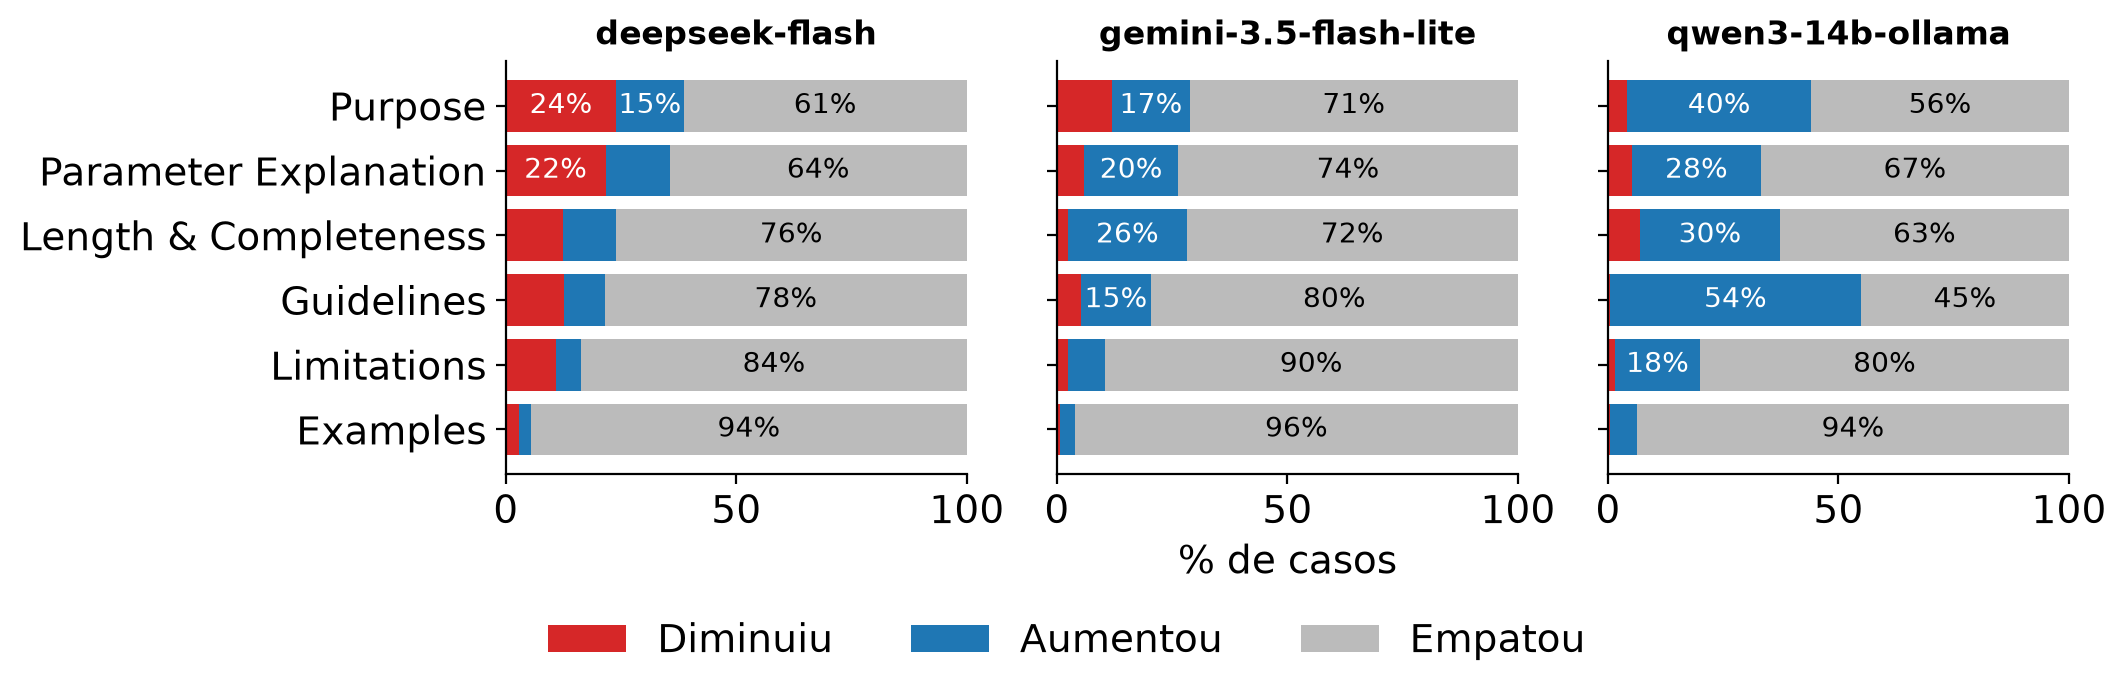
\includegraphics[width=0.95\linewidth]{images/RQs/diminuiu_empatou_aumentou_por_modelo.png}
    \caption{Distribuição proporcional da alteração nas pontuações por atributo e por juiz.}
    \label{fig:grafico_distribuicao}
\end{figure}

\begin{figure}[htbp]
    \centering
    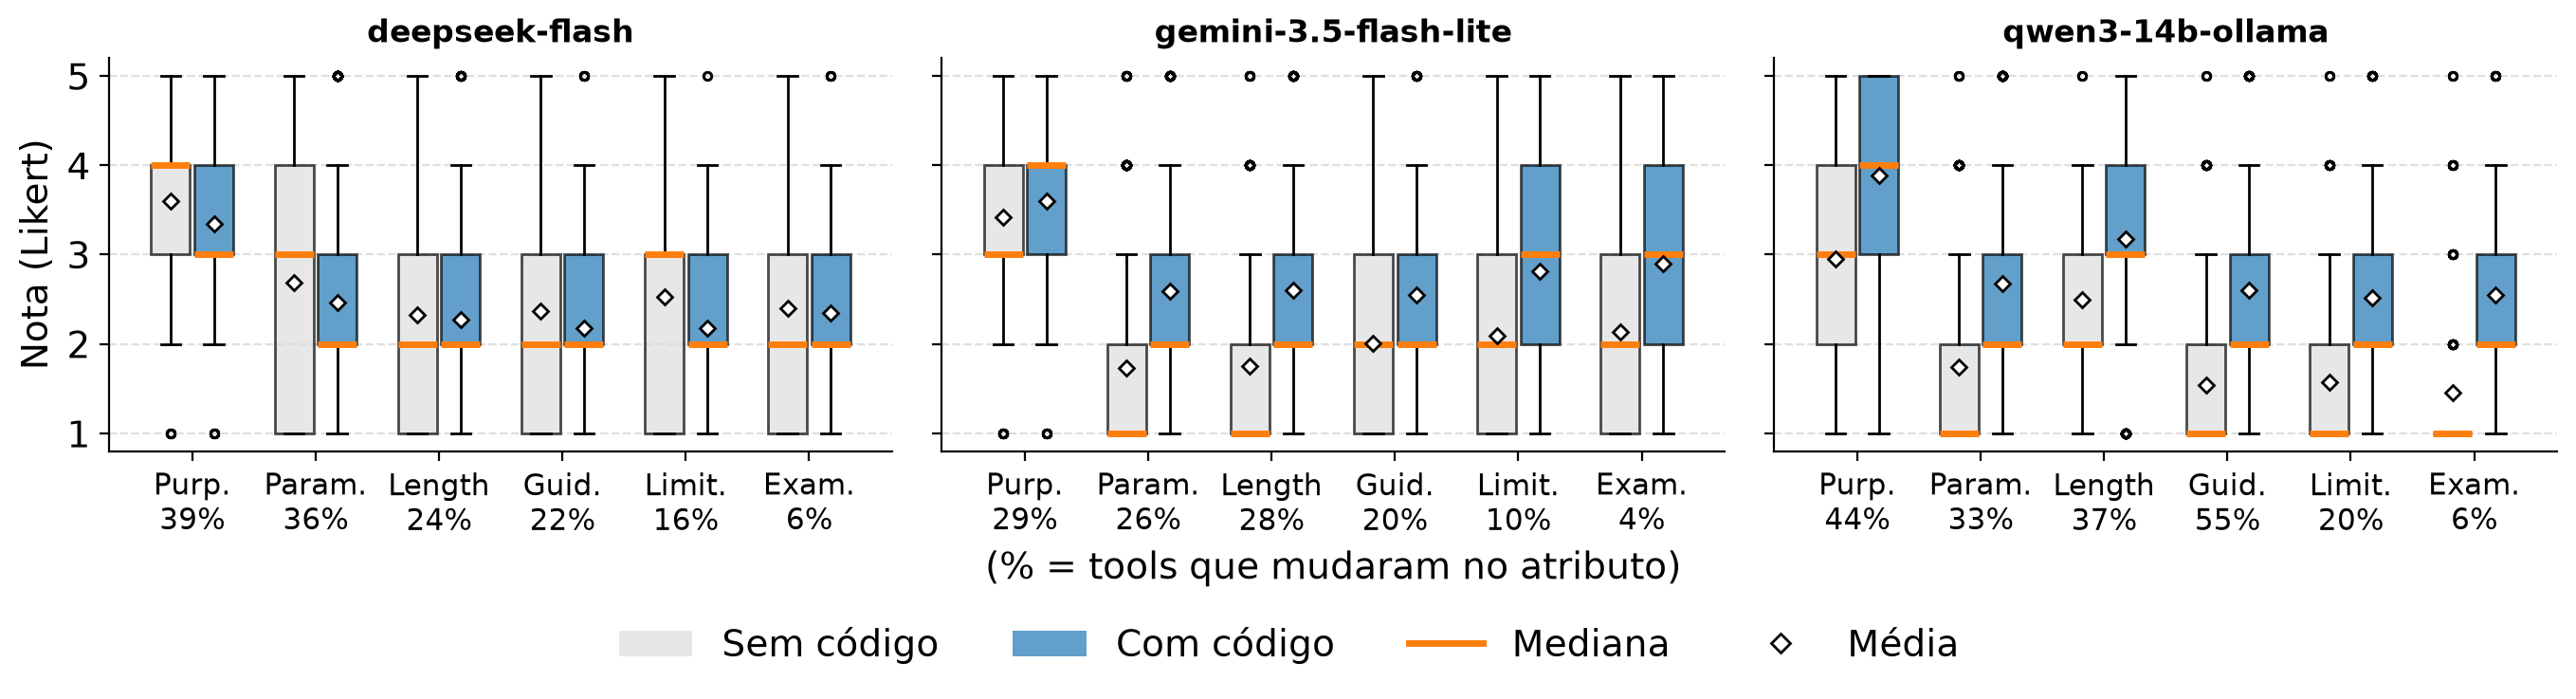
\includegraphics[width=0.95\linewidth]{images/RQs/boxplot_com_sem_codigo_apenas_mudou_por_modelo.png}
    \caption{Distribuição das notas nos cenários com e sem código, por juiz, considerando apenas os casos com alteração de pontuação (a maioria das avaliações empata, o que ocultaria a diferença).}
    \label{fig:boxplot}
\end{figure}

\textcolor{orange}{Três padrões se destacam. Primeiro, a direção da mudança depende do juiz: o DeepSeek tende a reduzir a nota com o código, com queda da média em todos os atributos e da mediana em \textit{Purpose}, \textit{Parameter Explanation} e \textit{Limitations}, enquanto Gemini e Qwen3 tendem a elevá-la, com média maior em todos os atributos e mediana maior em todos, exceto \textit{Guidelines} no Gemini; o Qwen3 apresenta as mudanças mais extremas, o que indica menor concordância com os outros dois juízes. Segundo, \textit{Purpose} é, em média, o atributo com maior variação, enquanto \textit{Limitations} e \textit{Examples} variam menos nos três juízes. Terceiro, \textit{Guidelines} destoa no Qwen3: é o único atributo em que os aumentos de nota superam os empates, embora seja o terceiro com menos variação no DeepSeek e no Gemini.}


\subsection{RQ3: As diferenças observadas entre os escores dos cenários com e sem código são estatisticamente significativas?}
\label{subsec:rq3}

\textcolor{orange}{A Tabela~\ref{tab:wilcoxon_media} reúne, por atributo, o resultado do Teste de Wilcoxon e da transição de quartil, ambos calculados sobre a média das notas dos três juízes (Seção~\ref{subsec:analise-comparativa}).}

\begin{table}[htbp]
\centering
\caption{Teste de Postos Sinalizados de Wilcoxon e transição de quartil das notas com e sem código, por atributo (média dos três juízes; pareado por \textit{tool}). $n$: pares com diferença não nula; faixas de quartil definidas pela distribuição sem código.}
\label{tab:wilcoxon_media}
\label{tab:transicao_quartis_media}
\footnotesize
\setlength{\tabcolsep}{4pt}
\begin{tabular}{lrrcrrr}
\toprule
 & \multicolumn{3}{c}{\textbf{Wilcoxon}} & \multicolumn{3}{c}{\textbf{Quartil}} \\
\cmidrule(lr){2-4} \cmidrule(lr){5-7}
\textbf{Atributo} & $n$ & $W$ & $p$-valor & Manteve & Subiu & Desceu \\
\midrule
Purpose & 7675 & 8576765,0 & $1,49 \times 10^{-224}$ & 68,2\% & 21,6\% & 10,2\% \\
Parameter Explanation & 7102 & 7716300,5 & $5,79 \times 10^{-178}$ & 65,7\% & 26,3\% & 8,1\% \\
Length \& Completeness & 6817 & 3788033,5 & $< 10^{-300}$ & 65,4\% & 28,5\% & 6,0\% \\
Guidelines & 7639 & 3721414,0 & $< 10^{-300}$ & 61,0\% & 37,7\% & 1,4\% \\
Limitations & 3365 & 1385458,5 & $8,40 \times 10^{-148}$ & 84,2\% & 13,1\% & 2,7\% \\
Examples & 1261 & 151287,0 & $1,44 \times 10^{-82}$ & 95,5\% & 3,9\% & 0,6\% \\
\bottomrule
\end{tabular}
\end{table}

\textcolor{orange}{Os seis atributos apresentam diferenças estatisticamente significativas entre os cenários ($p < 0{,}05$). Como o número de pares é elevado, até diferenças pequenas tendem a ser significativas, e a transição de quartil ajuda a dimensioná-las: \textit{Purpose}, \textit{Parameter Explanation}, \textit{Length \& Completeness} e \textit{Guidelines} mudam de faixa em 31,8\%, 34,4\%, 34,5\% e 39,1\% das ferramentas, respectivamente, enquanto \textit{Limitations} e \textit{Examples} mudam em apenas 15,8\% e 4,5\%. Esses dois atributos são também os que têm menos pares com nota alterada ($n$), e, em todos os atributos, subir de faixa é mais frequente do que descer.}

% Pré-preenchimento: revisar antes da entrega.
\section{Ameaças à Validade}
\label{sec:ameacas}

\textcolor{orange}{\textbf{Validade de construto.} Não há, neste estudo, um padrão-ouro humano de qualidade das descrições: a precisão da avaliação é inferida a partir do mecanismo pelo qual a nota muda (RQ1), não medida contra um julgamento de referência. Assim, demonstra-se que a mudança de nota tem causa identificável no código, mas não que a nota resultante seja, em sentido absoluto, mais correta. Além disso, tanto as avaliações quanto as etapas da análise qualitativa (síntese das justificativas, indução de categorias e classificação) são conduzidas por LLMs, e a verificação manual compara a categoria atribuída com a justificativa sintetizada e o \textit{reasoning} dos juízes, não diretamente com o código-fonte. O Gemini 3.5 Flash-Lite atua como juiz e também como sintetizador das justificativas, o que pode favorecer a sua própria leitura dos casos.}

\textcolor{orange}{\textbf{Validade interna.} O código fornecido ao avaliador é obtido por uma heurística de resolução de chamadas baseada em nome, não em tipos, limitada a três níveis de profundidade e a 32.000 caracteres (Apêndice~\ref{apendice:secao}). Parte da lógica relevante pode, portanto, ficar de fora, ou trechos de funções homônimas podem ser incluídos por engano, embora resoluções ambíguas sejam sinalizadas. As respostas dos juízes não são determinísticas, e a classificação das justificativas em categorias foi confirmada em 72\% da amostra verificada, com discordâncias concentradas entre categorias de fronteira próxima. Por outro lado, a amostra de divergência confirmada exige que todos os juízes concordem que a nota mudou, o que a torna conservadora frente ao ruído de um juiz isolado.}

\textcolor{orange}{\textbf{Validade externa.} A amostra restringe-se a 206 repositórios públicos do GitHub com ao menos 100 estrelas, concentrados em Python e TypeScript, e três repositórios respondem por 46,6\% das ferramentas, o que pode enviesar resultados agregados. Os resultados também refletem três modelos específicos em uma versão e momento determinados; como os próprios juízes divergem na direção do efeito (RQ2), não é possível generalizar o comportamento observado para outros avaliadores.}

\textcolor{orange}{\textbf{Validade de conclusão.} Com milhares de pares por atributo, até diferenças pequenas resultam em $p$-valores muito baixos; por isso, o Teste de Wilcoxon é acompanhado da transição de quartil, que dimensiona o efeito. Não foi aplicada correção para comparações múltiplas, mas, como todos os $p$-valores são inferiores a $10^{-80}$, uma correção de Bonferroni para seis testes ($\alpha = 0{,}0083$) não alteraria nenhuma conclusão. Por fim, a média entre juízes, usada na RQ3, pode atenuar efeitos de sentidos opostos, como a redução de notas pelo DeepSeek frente ao aumento pelo Gemini e pelo Qwen3, razão pela qual a RQ2 apresenta os resultados por juiz.}

% Pré-preenchimento: revisar antes da entrega.
\section{Conclusão e Trabalhos Futuros}
\label{sec:conclusao}

\textcolor{orange}{Este trabalho investigou se a avaliação da qualidade de descrições de ferramentas MCP é influenciada pela disponibilização do código da ferramenta ao avaliador. Para isso, 12.171 ferramentas de 206 servidores MCP foram extraídas, junto com o código alcançado por sua árvore de chamadas, e avaliadas por três LLMs segundo a rubrica de seis componentes de Hasan et al. (2026)\nocite{2026arXiv260214878M}, com e sem acesso ao código.}

\textcolor{orange}{Quanto à RQ1, na maior parte da amostra de divergência confirmada (89,2\%) a mudança de nota decorre de um achado concreto no código, sobretudo parâmetros e opções não documentados, modos de falha não divulgados e detalhes da estrutura de saída; isso é consistente com um ganho de precisão, embora não o comprove sem um padrão-ouro humano. Quanto à RQ2, a direção do efeito depende do juiz: o DeepSeek tende a reduzir as notas, enquanto o Gemini e o Qwen3 tendem a elevá-las; \textit{Purpose} é o atributo mais afetado e \textit{Limitations} e \textit{Examples} os menos afetados. Quanto à RQ3, as diferenças são estatisticamente significativas nos seis atributos, com mudança de faixa de quartil entre 31,8\% e 39,1\% das ferramentas em \textit{Purpose}, \textit{Parameter Explanation}, \textit{Length \& Completeness} e \textit{Guidelines}.}

\textcolor{orange}{Conclui-se que o código altera de forma consistente a avaliação das descrições e que essa alteração, na maioria dos casos, tem origem em informações que a descrição omite. A principal contribuição do trabalho é mostrar que avaliar descrições MCP isoladamente deixa de captar uma parcela relevante de suas deficiências, e oferecer uma caracterização empírica, em 16 categorias, do tipo de informação que o código revela.}

\textcolor{orange}{Como trabalhos futuros, propõe-se: (i) construir um padrão-ouro humano sobre uma amostra de ferramentas, permitindo medir diretamente se a avaliação com código é mais precisa; (ii) verificar se as deficiências reveladas pelo código afetam o desempenho real de agentes, por exemplo em \textit{benchmarks} baseados em execução como o MCP-Universe \cite{2025arXiv250814704L}; (iii) usar o código para reescrever automaticamente as descrições e avaliar o ganho de qualidade resultante; (iv) medir a concordância entre avaliadores na análise qualitativa, com um segundo codificador independente e o coeficiente Kappa por categoria; e (v) aprimorar a extração do código, com resolução de chamadas baseada em tipos e profundidade adaptativa.}

\bibliographystyle{sbc}
\bibliography{sbc-template}

 \appendix
 \section*{Apêndice}
 \section{Algoritmo de Construção do Grafo de Chamadas e Composição do Contexto de Código}
\label{apendice:secao}

Este apêndice detalha o algoritmo desenvolvido para a construção do grafo de
chamadas (\textit{call graph}) de cada ferramenta MCP e para a composição do
trecho de \textcolor{orange}{código} usado como contexto adicional no cenário de avaliação
que inclui \textcolor{orange}{código} (Seção~\ref{sec:materiais}). O algoritmo é
heurístico e baseado em análise estática via tree-sitter: a partir da função
que implementa a própria ferramenta, resolve por nome as chamadas feitas
dentro dela, até três níveis de profundidade, distinguindo chamadas
resolvidas dentro do próprio repositório de chamadas externas ou
dinamicamente determinadas, conforme ilustrado na Figura~\ref{fig:codigoarvore}.

\subsection*{Procedimento de Extração}
O algoritmo opera em três fases distintas, executadas uma vez por repositório:

\begin{enumerate}
    \item \textbf{Indexação estática do repositório:} são construídos, a
    partir de todo o \textcolor{orange}{código} do repositório, um índice de definições
    (nome simples e nome qualificado, \texttt{Classe.método}, de toda
    função/método encontrado, com referência ao seu corpo) e, por arquivo,
    um índice de \textit{imports} (alias local usado no arquivo
    $\rightarrow$ módulo e nome original de onde veio). Ambos são
    heurísticas de escopo léxico, não uma resolução completa de símbolos.

    \item \textbf{Construção recursiva do grafo de chamadas:} a árvore de
    cada ferramenta é construída a partir da função que a implementa
    (nível~1). Para cada chamada encontrada no corpo de uma função, uma
    heurística de resolução por nome é aplicada em ordem, valendo a
    primeira que casar: (i) receptor \texttt{self}/\texttt{this}
    $\rightarrow$ método da própria classe; (ii) mesmo nome definido no
    mesmo arquivo $\rightarrow$ função auxiliar local; (iii) receptor casa
    com um alias de \textit{import} conhecido $\rightarrow$ busca no
    módulo importado; (iv) nome único em todo o repositório
    $\rightarrow$ resolve diretamente; (v) não encontrado em lugar nenhum
    (biblioteca externa, \textit{stdlib}, ou chamada genuinamente
    dinâmica) $\rightarrow$ tratado como folha externa, sem recursão.
    Uma chamada resolvida vira um novo nó, expandido recursivamente até o
    nível~3; nós de nível~3 continuam sendo chamadas normalmente
    resolvidas, mas suas próprias chamadas internas não são mais
    exploradas. Esse limite é uma decisão de engenharia: contém o tamanho
    da árvore a um custo previsível e elimina, por construção, qualquer
    risco de laço infinito em recursão direta ou mútua, sem exigir
    detecção de ciclo separada. Quando mais de um candidato válido é encontrado num mesmo
    passo (nome duplicado em escopos distintos), o desempate é feito pela
    menor distância de diretório até o arquivo de origem da chamada, e o
    nó resultante permanece explicitamente sinalizado como \textit{ambíguo}
    na estrutura de dados, em vez de ser tratado como uma resolução certa.

    \item \textbf{Composição do contexto de código:} no cenário de
    avaliação que inclui \textcolor{orange}{código}, a árvore é percorrida em
    pré-ordem e, para cada nó resolvido, o trecho de \textcolor{orange}{código}
    correspondente (linhas de início e fim exatas) é lido diretamente do
    repositório clonado em disco e anotado com um comentário indicando o
    nível na árvore, a chamada de origem e a localização exata
    (arquivo:linhas). Nós externos/não resolvidos entram apenas como um
    comentário sinalizando a chamada não resolvida, sem trecho de código.
    Os trechos são concatenados na ordem de visita; o texto resultante é
    limitado a 32.000 caracteres antes de ser enviado ao
    avaliador, para conter o custo e a atenção do modelo: um corte por
    tamanho, não uma sumarização do conteúdo.
\end{enumerate}

\section{Prompts Utilizados na Análise Qualitativa das Divergências}
\label{apendice:secao-prompts}

Este apêndice reproduz, na íntegra e no idioma original (inglês, mesmo idioma em que a justificativa de cada juiz é produzida), os três \textit{prompts} de sistema (\textit{system instruction}) utilizados nas três etapas da análise qualitativa descrita na Seção~\ref{subsec:analise-comparativa}. Em todos os casos, o modelo recebe o \textit{prompt} de sistema reproduzido abaixo e, na mensagem do usuário, o objeto ou lista JSON de entrada descrito no próprio texto do \textit{prompt}; a saída é restrita a um objeto ou lista JSON, sem texto adicional, por meio do mecanismo de saída estruturada do respectivo modelo: Gemini nas Etapas 1 e 3, e DeepSeek na Etapa 2.

\subsection*{Etapa 1: Geração de Justificativas}

Aplicado individualmente a cada ferramenta da amostra de divergência confirmada (Seção~\ref{subsec:consolidacao}), recebendo como entrada um objeto JSON com os campos \texttt{tool\_uid}, \texttt{tool\_name}, a lista \texttt{avaliacoes} (uma entrada por juiz e cenário, já restrita aos componentes da rubrica cuja nota divergiu) e \texttt{source\_code}.

\begin{lstlisting}[language={}, breaklines=true, basicstyle=\small\ttfamily, caption=Prompt de sistema -- geração de justificativas, label=prompt:justificativas]
You are a research assistant helping analyze results from an undergraduate thesis ("Model Context Protocol (MCP): Avaliação da Qualidade de Descrições de Tools com Base em Contexto de Código-Fonte") that studies whether giving an LLM-as-judge access to a tool's source code changes its evaluation of the tool's natural-language description. Several judge models independently scored the SAME description on a 1-5 Likert scale across 6 rubric components (Purpose, Guidelines, Limitations, Parameter Explanation, Length & Completeness, Examples), once without the source code ("description_only") and once with it ("with_source"). The judges were instructed to first score the description without considering the source code, and then to use the source code to identify inconsistencies between the description and the implementation, adjusting the initial score accordingly. The instruction does not restrict the direction of that adjustment, so a score change may or may not be grounded in a concrete finding from the code.

You will receive one JSON object describing a single tool for which at least one component's score changed between the two scenarios, for every judge that evaluated it unanimously. It has:
- "tool_uid": a unique identifier for the tool.
- "tool_name": the tool's name.
- "avaliacoes": a list of per-judge, per-scenario entries. Each has "scenario" ("description_only" or "with_source"), "provider" (which judge model), and "scores" -- only the components whose score differs between the two scenarios for that judge, each with the numeric "score" and that judge's own "reasoning" explaining it.
- "source_code": the actual source snippet(s) the "with_source" judges saw.

Task: read every judge's reasoning for its changed component(s), cross-reference it against "source_code", and write ONE justification (3-5 sentences) explaining WHAT the source code revealed that the plain-text description did not -- e.g. an undocumented parameter, an undisclosed behavior/output, a missing limitation or error case, or a direct contradiction between the description and the implementation. If judges disagree on the reason, or if a judge's reasoning gives no concrete evidence from the code (just a vaguer/stricter reading of the same text), say so plainly instead of inventing a justification.

Ground every claim in specific details from the reasoning and/or the source code. Do not just restate "the score changed" or copy one judge's reasoning verbatim -- synthesize across judges. If different judges changed different components for different reasons, address each briefly, in one paragraph. Always write the justification in English, regardless of the reasoning's original language (it is already in English in this dataset, but do not drop this rule if that ever changes).

Be conservative per component: a strong, well-evidenced finding for one judge/component (e.g. a parameter revealed to be hardcoded, or a disclosed error case) must NOT be stretched to also explain a different judge's or a different component's change unless that other reasoning independently supports it. When a specific score change's reasoning is vague or generic (e.g. "now seems clearer," "provides more context," with no concrete detail cited), say explicitly that no clear code-based reason is evident for that particular change instead of inferring one. Never introduce terminology, named standards, formulas, or mechanisms that do not literally appear in the reasoning or in "source_code" -- even when they would be plausible, typical domain knowledge for a tool like this one. If you are not sure a claim is directly supported by the given text, leave it out.

Output ONLY one JSON object, no text before or after it, in exactly this shape:
{"tool_uid": "<the tool_uid from the input, verbatim>", "justification": "<your justification>"}
\end{lstlisting}

\subsection*{Etapa 2: Identificação Indutiva de Categorias}

Aplicado uma única vez, recebendo como entrada o conjunto completo de justificativas produzidas na Etapa 1, no formato de uma lista JSON de objetos \texttt{\{"tool\_uid": ..., "justification": ...\}}.

\begin{lstlisting}[language={}, breaklines=true, basicstyle=\small\ttfamily, caption=Prompt de sistema -- identificação indutiva de categorias, label=prompt:categorias]
You are a qualitative research assistant conducting a thematic analysis for an undergraduate thesis ("Model Context Protocol (MCP): Avaliação da Qualidade de Descrições de Tools com Base em Contexto de Código-Fonte") that studies whether giving an LLM-as-judge access to a tool's source code changes its evaluation of the tool's natural-language description. For every tool where every judge that evaluated it changed at least one rubric score between the "description_only" and "with_source" scenarios, a short English justification was already written, explaining WHAT the source code revealed that the plain-text description did not.

You will receive a JSON array of {"tool_uid": ..., "justification": ...} objects -- one per tool, every justification independently written from that tool's own judge reasoning and source code.

Task: perform an inductive thematic analysis (open coding, following Braun & Clarke's six-phase method: familiarization, initial coding, searching for themes, reviewing themes, defining and naming themes) across ALL justifications to identify the recurring categories of WHAT KIND of thing the source code tends to reveal that the description does not. Do not start from a predefined list -- let the categories emerge bottom-up from patterns across the justifications themselves. Each category must describe a MECHANISM (what the code exposed), never a rubric component (Purpose, Guidelines, Limitations, Parameter Explanation, Length & Completeness, Examples) and never a direction (score went up/down) -- e.g. "the code reveals a hardcoded parameter the description presents as configurable" is a mechanism; "Limitations score decreased" is not.

Requirements for the final set of categories:
- Between 5 and 15 categories. Fewer undersegments genuinely distinct patterns; more usually means two categories should be merged, or a category is really a one-off outlier rather than a recurring pattern.
- Each category must be grounded in multiple justifications across different tools -- never create a category for a single idiosyncratic case.
- Categories must be mutually distinguishable: if two candidate categories would classify the same justification the same way almost every time, merge them into one.
- Name each category concisely (2-5 words, a short analytic label, Title Case).
- Each description must state, in 2-3 sentences: (a) what the category captures, in terms of the specific kind of discrepancy or disclosure found in the code, and (b) one illustrative, paraphrased example pattern drawn from the justifications -- never quote or name a specific tool_uid.

Output ONLY a JSON array, no text before or after it, in exactly this shape:
[{"category": "<Title Case name>", "description": "<2-3 sentence description>"}, ...]

Write everything in English.
\end{lstlisting}

\subsection*{Etapa 3: Classificação Dedutiva por Categoria}

Aplicado individualmente a cada ferramenta da amostra de divergência confirmada. O trecho reproduzido como \texttt{<lista de categorias da Etapa 2, uma por linha>} é substituído, em tempo de execução, pela lista de categorias produzida na Etapa 2 (nome e descrição de cada uma); \texttt{"none"} é a categoria de reserva explícita, utilizada quando nenhuma das categorias da lista fixa corresponde à justificativa analisada.

\begin{lstlisting}[language={}, breaklines=true, basicstyle=\small\ttfamily, caption=Prompt de sistema -- classificação dedutiva por categoria, label=prompt:categorizacao]
You are a qualitative research assistant performing directed content analysis for an undergraduate thesis ("Model Context Protocol (MCP): Avaliação da Qualidade de Descrições de Tools com Base em Contexto de Código-Fonte") that studies whether giving an LLM-as-judge access to a tool's source code changes its evaluation of the tool's natural-language description.

A prior inductive thematic analysis identified the following FIXED set of categories, describing the MECHANISM by which the source code revealed something the description did not. Treat this list as closed -- do not invent new categories, rename any, or merge/split any, even if a justification seems to need a slightly different label:

<lista de categorias da Etapa 2, uma por linha>

You will receive one JSON object: {"tool_uid": ..., "justification": ...}. Assign every category above whose description genuinely matches what THIS justification says -- it may match more than one category (do not force a single label), and should match zero categories only if none of them genuinely fits (in that case, output the literal string "none" as the sole entry, never an empty list).

Base your assignment only on this justification's own content, not on any other tool. Output ONLY one JSON object, no text before or after it, in exactly this shape:
{"tool_uid": "<copied verbatim from the input>", "categories": ["<matching category name(s), or \"none\">"]}
\end{lstlisting}


\end{document}
